\documentclass[a4paper,10pt,twoside]{article}

\usepackage[top=1in, bottom=1in, left=1in, right=1in]{geometry}
\usepackage[utf8]{inputenc}
\usepackage[spanish,es-ucroman,es-noquoting]{babel}
\usepackage{setspace}
\usepackage{fancyhdr}
\usepackage{lastpage}
\usepackage{amsmath}
\usepackage{amsfonts}
\usepackage{verbatim}
\usepackage{listings}
\usepackage{graphicx}
\usepackage{float}
\usepackage{algorithmic}
\usepackage{color}
\usepackage{hyperref}
\usepackage[usenames,dvipsnames]{xcolor}
\definecolor{dkgreen}{rgb}{0,0.6,0}
\definecolor{gray}{rgb}{0.97,0.97,0.97}
\definecolor{mauve}{rgb}{0.58,0,0.82}
\usepackage{tikz}
\usetikzlibrary{calc}
\usetikzlibrary{decorations.pathreplacing}


% Evita que el documento se estire verticalmente para ocupar
% el espacio vacío en cada página.
\raggedbottom


%%%%%%%%%% Configuración de Fancyhdr - Inicio %%%%%%%%%%
\pagestyle{fancy}
\thispagestyle{fancy}
\lhead{Trabajo Práctico 2, Organización del Computador II}
\rhead{Chapresto, Rey, Vileriño}
\renewcommand{\footrulewidth}{0.4pt}
\cfoot{\thepage /\pageref{LastPage}}

\fancypagestyle{caratula} {
   \fancyhf{}
   \cfoot{\thepage /\pageref{LastPage}}
   \renewcommand{\headrulewidth}{0pt}
   \renewcommand{\footrulewidth}{0pt}
}
%%%%%%%%%% Configuración de Fancyhdr - Fin %%%%%%%%%%


%%%%%%%%%% Configuración de Algorithmic - Inicio %%%%%%%%%%
% Entorno propio para customizar la presentación del pseudocódigo
\newenvironment{pseudocodigo}
    {\vspace{0.5em} \begin{algorithmic}}
    {\end{algorithmic} \vspace{0.5em}}

% Alinear comentarios a la derecha
\renewcommand{\algorithmiccomment}[1]{\hfill \{#1\}}
%%%%%%%%%% Configuración de Algorithmic - Fin %%%%%%%%%%


%%%%%%%%%% Macros de tikz - Inicio %%%%%%%%%%
% Uso: \registroCuatro{etiqueta}{x}{y}{a4}{a3}{a2}{a1}
\newcommand{\registroCuatro}[7]{
    \ifthenelse{\equal{#1}{}}{}{
        \draw (#2, {#3 + 0.5}) node[anchor=east]{#1};
    }

    \draw   (#2, #3) rectangle +(4, 1) +(2, 0.5) node{#4}
          ++(4, 0)   rectangle +(4, 1) +(2, 0.5) node{#5}
          ++(4, 0)   rectangle +(4, 1) +(2, 0.5) node{#6}
          ++(4, 0)   rectangle +(4, 1) +(2, 0.5) node{#7};          
}

% Uso: \registroOcho{etiqueta}{x}{y}{a8}{a7}{a6}...{a1}
\newcommand{\registroOcho}[9]{
    \def\etiqueta{#1}
    \def\x{#2}
    \def\y{#3}
    \def\aviii{#4}
    \def\avii{#5}
    \def\avi{#6}
    \def\av{#7}
    \def\aiv{#8}
    \def\aiii{#9}
    \registroOchoX    
}
\newcommand{\registroOchoX}[2]{ % Auxiliar - no usar directamente
    \def\aii{#1}
    \def\ai{#2}
    \ifthenelse{\equal{\etiqueta}{}}{}{
        \draw (\x, {\y + 0.5}) node[anchor=east]{\etiqueta};
    }
    \filldraw[fill=white]
        (\x, \y) rectangle +(2, 1) +(1, 0.5) node{\aviii}
        ++(2, 0) rectangle +(2, 1) +(1, 0.5) node{\avii}
        ++(2, 0) rectangle +(2, 1) +(1, 0.5) node{\avi}
        ++(2, 0) rectangle +(2, 1) +(1, 0.5) node{\av}
        ++(2, 0) rectangle +(2, 1) +(1, 0.5) node{\aiv}
        ++(2, 0) rectangle +(2, 1) +(1, 0.5) node{\aiii}
        ++(2, 0) rectangle +(2, 1) +(1, 0.5) node{\aii}
        ++(2, 0) rectangle +(2, 1) +(1, 0.5) node{\ai};
}


% Uso: \registroDieciseis{etiqueta}{x}{y}{a16}{a15}{a14}...{a1}
\newcommand{\registroDieciseis}[9]{
    \def\etiqueta{#1}
    \def\x{#2}
    \def\y{#3}
    \def\axvi{#4}
    \def\axv{#5}
    \def\axiv{#6}
    \def\axiii{#7}
    \def\axii{#8}
    \def\axi{#9}
    \registroDieciseisX
}
\newcommand{\registroDieciseisX}[9]{ % Auxiliar - no usar directamente
    \def\ax{#1}
    \def\aix{#2}
    \def\aviii{#3}
    \def\avii{#4}
    \def\avi{#5}
    \def\av{#6}
    \def\aiv{#7}
    \def\aiii{#8}
    \def\aii{#9}
    \registroDieciseisXX
}
\newcommand{\registroDieciseisXX}[1]{ % Auxiliar - no usar directamente
    \def\ai{#1}
    \ifthenelse{\equal{\etiqueta}{}}{}{
        \draw (\x, {\y + 0.5}) node[anchor=east]{\etiqueta};
    }
    \filldraw[fill=white]
        (\x, \y) rectangle +(1, 1) +(0.5, 0.5) node{\axvi}
        ++(1, 0) rectangle +(1, 1) +(0.5, 0.5) node{\axv}
        ++(1, 0) rectangle +(1, 1) +(0.5, 0.5) node{\axiv}
        ++(1, 0) rectangle +(1, 1) +(0.5, 0.5) node{\axiii}
        ++(1, 0) rectangle +(1, 1) +(0.5, 0.5) node{\axii}
        ++(1, 0) rectangle +(1, 1) +(0.5, 0.5) node{\axi}
        ++(1, 0) rectangle +(1, 1) +(0.5, 0.5) node{\ax}
        ++(1, 0) rectangle +(1, 1) +(0.5, 0.5) node{\aix}
        ++(1, 0) rectangle +(1, 1) +(0.5, 0.5) node{\aviii}
        ++(1, 0) rectangle +(1, 1) +(0.5, 0.5) node{\avii}
        ++(1, 0) rectangle +(1, 1) +(0.5, 0.5) node{\avi}
        ++(1, 0) rectangle +(1, 1) +(0.5, 0.5) node{\av}
        ++(1, 0) rectangle +(1, 1) +(0.5, 0.5) node{\aiv}
        ++(1, 0) rectangle +(1, 1) +(0.5, 0.5) node{\aiii}
        ++(1, 0) rectangle +(1, 1) +(0.5, 0.5) node{\aii}
        ++(1, 0) rectangle +(1, 1) +(0.5, 0.5) node{\ai};
}
%%%%%%%%%% Macros de tikz - Fin %%%%%%%%%%


%%%%%%%%%% Macros misceláneos - Inicio %%%%%%%%%%
\newcommand{\xmm}[1]{\texttt{XMM#1}}
\newcommand{\rax}{\texttt{RAX}}
\newcommand{\rbx}{\texttt{RBX}}
\newcommand{\rcx}{\texttt{RCX}}
\newcommand{\rdx}{\texttt{RDX}}
\newcommand{\rbp}{\texttt{RBP}}
\newcommand{\rsp}{\texttt{RSP}}
\newcommand{\reg}[1]{\texttt{R#1}}
\newcommand{\asm}[1]{\texttt{\uppercase{#1}}}
%%%%%%%%%% Macros misceláneos - Fin %%%%%%%%%%


\begin{document}


%%%%%%%%%%%%%%%%%%%%%%%%%%%%%%%%%%%%%%%%%%%%%%%%%%%%%%%%%%%%%%%%%%%%%%%%%%%%%%%
%% Carátula                                                                  %%
%%%%%%%%%%%%%%%%%%%%%%%%%%%%%%%%%%%%%%%%%%%%%%%%%%%%%%%%%%%%%%%%%%%%%%%%%%%%%%%


\thispagestyle{caratula}

\begin{center}


\includegraphics[height=2cm]{DC.png} 
\hfill

\includegraphics[height=2cm]{UBA.jpg} 

\vspace{2cm}

Departamento de Computación,\\
Facultad de Ciencias Exactas y Naturales,\\
Universidad de Buenos Aires

\vspace{4cm}

\begin{Huge}
Trabajo Práctico 2
\end{Huge}

\vspace{0.5cm}

\begin{Large}
Organización del Computador II
\end{Large}

\vspace{1cm}

Segundo Cuatrimestre de 2013

\vspace{4cm}

Grupo: \textbf{Crema Americana/Persico}

\vspace{0.5cm}

\begin{tabular}{|c|c|c|}
    \hline
    Apellido y Nombre & LU & E-mail\\
    \hline
    Silvio Vileriño             & 106/12 & svilerino@gmail.com\\
    Esteban Rey 				& 657/10 & estebanlucianorey@gmail.com\\
    Matias Chapresto 			& 201/12 & matiaschapresto@gmail.com\\
    \hline
\end{tabular}

\vspace{1cm}

\textbf{PC utilizada para las mediciones:} \\
\vspace{0.cm}
\begin{tabular}{|c|c|}
    \hline
    CPU &   Sandy Bridge Core i5-2500k @3.30Ghz\\
    \hline
    GPU & AMD Radeon 7800 HD\\
    \hline
    Mem.    &   8Gb Ddr3    \\
    \hline
\end{tabular}

\end{center}

\newpage


%%%%%%%%%%%%%%%%%%%%%%%%%%%%%%%%%%%%%%%%%%%%%%%%%%%%%%%%%%%%%%%%%%%%%%%%%%%%%%%
%% Índice                                                                    %%
%%%%%%%%%%%%%%%%%%%%%%%%%%%%%%%%%%%%%%%%%%%%%%%%%%%%%%%%%%%%%%%%%%%%%%%%%%%%%%%


\tableofcontents

\newpage


%%%%%%%%%%%%%%%%%%%%%%%%%%%%%%%%%%%%%%%%%%%%%%%%%%%%%%%%%%%%%%%%%%%%%%%%%%%%%%%
%% Introducción                                                              %%
%%%%%%%%%%%%%%%%%%%%%%%%%%%%%%%%%%%%%%%%%%%%%%%%%%%%%%%%%%%%%%%%%%%%%%%%%%%%%%%


\section{Introducción}
El objetivo de este trabajo practico explorar y realizar experimentos sobre la tecnologia Streaming SIMD extensions provista por Intel que promete optimizar procesamientos que sean iguales para una cantidad multiple de datos.\\
Con este objetivo en mente, realizaremos varias implementaciones de 3 filtros, 2 sobre videos y uno sobre imagenes, considerando una implementacion en lenguaje C y otra en lenguaje Assembler utilizando las instrucciones brindadas por el set de instrucciones SIMD. Esperamos obtener mejoras respecto a rendimiento. Realizaremos una serie de experimentos y analisis sobre cada filtro y a continuacion de estos escribiremos conclusiones sobre los datos obtenidos.


%%%%%%%%%%%%%%%%%%%%%%%%%%%%%%%%%%%%%%%%%%%%%%%%%%%%%%%%%%%%%%%%%%%%%%%%%%%%%%%
%% Desarrollo                                                                %%
%%%%%%%%%%%%%%%%%%%%%%%%%%%%%%%%%%%%%%%%%%%%%%%%%%%%%%%%%%%%%%%%%%%%%%%%%%%%%%%


\section{Desarrollo}

\subsection{Filtro Color}

El filtro color consiste en realizar una iteracion sobre los pixeles de una imagen, estos se dividen en 3 componentes, cada una de ellas identifica un color de la codificacion RGB de la imagen. La iteracion del filtro deja sin modificaciones
los pixeles cuya distancia euclideana de sus componentes se encuentren dentro de un rango especificado por el par\'ametro threshold,los pixeles que no cumplan dicha condicion, se convertiran a blanco y negro por medio de una conversion basada en dejar las 3 componentes del pixel con el promedio de dichas componentes originales.
\\
\\
Como en esta ocasi\'on estamos trabajando con archivos de video, los cuales se pueden definir como una secuencia
de im\'agenes o frames. El filtro aplicar\'a frame por frame la operatoria explicada arriba como si fueran im\'agenes.
\\
\\
Dado que el objetivo de este trabajo pr\'actico es explorar el modelo de procesamiento SIMD que provee Intel, por este motivo se produjeron 2 implementaciones, una en lenguaje C, y la otra en ASM de 64 bits utilizando instrucciones SIMD.
\\

%%%%%%%%%%%%%%%%%%%%%%%%%%%%%%%%%%%%%%%%%%%%%%%%%%%%%%%%%%%%%%%%%%%%%%%%%%%%%%%
%% Descripción del ciclo                                                     %%
%%%%%%%%%%%%%%%%%%%%%%%%%%%%%%%%%%%%%%%%%%%%%%%%%%%%%%%%%%%%%%%%%%%%%%%%%%%%%%%

\subsubsection{Descripción del algoritmo}

Veamos la implementacion en C y utilizemosla como pseudocodigo para explicar el filtro:\\
Para cada frame del video de entrada, se realiza el siguiente algoritmo:\\

\lstinputlisting[language=C,tabsize=4, numbers=left, numberstyle=\tiny\color{black},mathescape=true, backgroundcolor=\color{gray}, rulecolor=\color{black}, keywordstyle=\color{blue}, commentstyle=\color{dkgreen},stringstyle=\color{mauve}, numbersep=5pt, basicstyle=\scriptsize]{fuentes/pseudocolor_filter_c.c}

\textbf{Explicacion del algoritmo:}\\ Dividamos en secciones el algoritmo en secciones y analicemos en detalle una por una.\\

\begin{enumerate}
    \item \textbf{Declaracion de variables : Lineas 15-25} \\
      Declaramos afuera del ciclo las variables que vamos a utilizar para el procesamiento.

    \item \textbf{Lectura de un pixel como 3 bytes desde la imagen origen : Lineas 26-30}\\
      Obtenemos de memoria los 3 bytes que corresponden a los colores azul, verde y rojo de un pixel.
      En la Figura se indica la lectura de este pixel.\\
      
      \par      
      \bigskip
        \begin{tikzpicture}
            [>=latex,font=\sffamily,every node/.style={minimum width=1cm,minimum height=1.5em,outer sep=0pt,draw=black,fill=blue!40,semithick}]
                    \node at (2, 0) (J) {var B};
                    \node at (4, 0) (L) {var R};
                    \node at (6, 0) (K) {var G};
            
            [>=latex,font=\sffamily,every node/.style={minimum width=1cm,minimum height=1.5em,outer sep=0pt,draw=black,fill=blue!40,semithick}]
                    \node at (1,4) (A) {...};
                    \node [anchor=west] at (A.east) (B) {B};
                    \node [anchor=west] at (B.east) (C) {G};
                    \node [anchor=west] at (C.east) (D) {R};
                    \node [anchor=west] at (D.east) (E) {...};
                    \node [anchor=west] at (E.east) (F) {B};
                    \node [anchor=west] at (F.east) (G) {G};
                    \node [anchor=west] at (G.east) (H) {R};
                    \node [anchor=west] at (H.east) (I) {...};

            
            %flechitas  
            \draw [->,shorten >=2pt,shorten <=2pt,semithick] (B.south) -- +(0,-1em) -| (J.north);
            \draw [->,shorten >=2pt,shorten <=2pt,semithick] (D.south) -- +(0,-1em) -| (K.north);
            \draw [->,shorten >=2pt,shorten <=2pt,semithick] (C.south) -- +(0,-1em) -| (L.north);
        \end{tikzpicture}

        \par
        \bigskip
        \textbf{Figura:} Lectura de un pixel en 3 variables componentes.
    \item \textbf{Procesamiento para obtener la distancia euclidiana : Lineas 31-39}\\
      Realizamos las operaciones aritmeticas necesarias sobre las 3 componentes del pixel obteniendo la distancia euclidiana. Para esta seccion se realizaron algunas conversiones de datos, a continuacion de justificaran las elecciones de variables.
      \\
      \begin{itemize}
        \item \textbf{Almacenamiento en double words: }
        Como la diferencia de dos bytes no signados puede estar en el rango
        [-255,255] necesitamos un tamaño de datos mas grande para contener este
        resultado, por ejemplo signed short(word). Se eligio utilizar variables
        signadas double word, pues luego, cuando se calcula el cuadrado, dicho numero
        puede tomar como maximo el valor 65535, que no podria representarse en un word signado.
        La distancia se almacena en double word pues como maximo puede tomar el valor 3*65535.
      \end{itemize}
    \item \textbf{Comparacion y procesamiento correspondiente: Lineas 40 y 47}\\
      Se realiza la comparacion entre la distancia calculada y el parametro umbral dado como par\'ametro, se decide por cual de las siguientes 2 etapas continuar el procesamiento.
    \item \textbf{Procesamiento Caso 1: Lineas 41-46}\\
      Esta seccion es ejecutada en caso de que la distancia euclidiana este fuera del rango de filtrado. Puede caracterizarse por la transformacion a blanco y negro de los pixeles que sean procesados por esta seccion.
      La conversion se realiza por medio de el calculo del promedio de las componentes del color del pixel, y la posterior
      escritura de dicho pixel dejando el promedio en cada una de las 3 componentes.
      Para esta seccion se realizaron algunas conversiones de datos, a continuacion de justificaran las elecciones de variables.
      \\
      \begin{itemize}
        \item \textbf{Variable auxiliar promedio y reconversion a byte sin signo: }
        Se expreso la variable promedio como un word sin signo, ya que alcanza para almacenar la suma maxima de 3 bytes no signados.\\
        Utilizando el siguiente lema, podemos asegurar que el promedio de 3 bytes no signados puede almacenarse como byte no signado, lo que nos permite una conversion segura de word sin signo a byte sin signo.\\
        \textbf{Lema: } Sea $ A = \{a_1, a_2, a_3, ... a_n\} $ un conjunto de bytes sin signo. Luego vale que $promedio(A) \leq max(A)$.
      \end{itemize}
    \item \textbf{Procesamiento Caso 2: Lineas 48-50}\\
      Esta seccion es ejecutada en caso de que la distancia euclidiana se encuentre dentro del rango establecido por el umbral. Consiste en escribir en destino el pixel de la misma forma que fue leido, sin modificaciones.
           
\end{enumerate}

Luego de realizar el algoritmo en C, se le aplicaron una serie de optimizaciones, a saber:
\begin{enumerate}
  \item \textbf{Eliminacion de llamadas innecesarias dentro del ciclo:} 
          Una temprana implementacion del filtro contenia la logica de la distancia tal cual especificada en el enunciado, y se encontraba plasmada en una funcion auxiliar que recibia los parametros y devolvia la distancia.
          Con el fin de eliminar saltos innecesarios dentro del ciclo, se decidio introducir esta funcion dentro del ciclo.
  \item \textbf{Eliminacion del calculo de la raiz cuadrada en cada ciclo: }
          Una temprana implementacion calculaba la distancia y la comparaba con el parametro threshold (o umbral) pasado por parametro. Se decidio elevar al cuadrado ambos miembros de la desigualdad, de forma que con calcular $threshold^2$ fuera del ciclo, y comparar con la distancia al cuadrado, se reducia la cantidad de calculos aritmeticos realizados.
  \item \textbf{Declaracion de variables auxiliares(de pila) fuera del ciclo}
          Una temprana temprana implementacion declaraba las variables auxiliares dentro del ciclo, se decidio declararlas fuera, de forma que con una sola declaracion con un scope mas general de las mismas se puedan reutilizar.

\end{enumerate}

\subsubsection{Implementacion en assembler utilizando set de instrucciones SIMD}

Para realizar esta implementacion se tomo la idea general de la implementacion en C, 
pero dada la naturaleza de la implementacion de SIMD se eliminaron los saltos condicionales, y se utilizaron mascaras para procesar los casos de aplicacion del filtro sobre los pixeles.\\
Se procesaran 4 pixeles por ciclo.\\

Dividamos en secciones el codigo y expliquemos cada una de ellas.\\

\begin{itemize}
  \item \textbf{Declaracion de mascaras y precomputo de calculos auxiliares}

            \par      
            \bigskip
             \begin{figure}[!ht]
              \centering
                 \begin{tikzpicture}
                  \registroDieciseis{}{0}{5}
                   {255}{255}{255}{9} {255}{255}{255}{6}
                   {255}{255}{255}{3} {255}{255}{255}{0}
              \end{tikzpicture}
              \caption{Mascara de reordenamiento de canal azul}
            \end{figure}


            \par      
            \bigskip
             \begin{figure}[!ht]
              \centering
                 \begin{tikzpicture}
                  \registroDieciseis{}{0}{5}
                   {255}{255}{255}{10} {255}{255}{255}{7}
                   {255}{255}{255}{4} {255}{255}{255}{1}
              \end{tikzpicture}
              \caption{Mascara de reordenamiento de canal verde}
            \end{figure}


            \par      
            \bigskip
             \begin{figure}[!ht]
              \centering
                 \begin{tikzpicture}
                  \registroDieciseis{}{0}{5}
                   {255}{255}{255}{11} {255}{255}{255}{8}
                   {255}{255}{255}{5} {255}{255}{255}{2}
              \end{tikzpicture}
              \caption{Mascara de reordenamiento de canal rojo}
            \end{figure}

            \par      
            \bigskip
             \begin{figure}[!ht]
              \centering
                 \begin{tikzpicture}
                  \registroDieciseis{}{0}{5}
                   {255}{255}{255}{255} {255}{255}{12}{255}
                   {255}{8}{255}{255} {4}{255}{255}{0}
              \end{tikzpicture}
              \caption{Mascara de reordenamiento inversa de canal azul}
            \end{figure}

            \par      
            \bigskip
             \begin{figure}[!ht]
              \centering
                 \begin{tikzpicture}
                  \registroDieciseis{}{0}{5}
                   {255}{255}{255}{255} {255}{12}{255}{255}
                   {8}{255}{255}{4} {255}{255}{0}{255}
              \end{tikzpicture}
              \caption{Mascara de reordenamiento inversa de canal verde}
            \end{figure}

            \par      
            \bigskip
             \begin{figure}[!ht]
              \centering
                 \begin{tikzpicture}
                  \registroDieciseis{}{0}{5}
                   {255}{255}{255}{255} {12}{255}{255}{8}
                   {255}{255}{4}{255} {255}{0}{255}{255}
              \end{tikzpicture}
              \caption{Mascara de reordenamiento inversa de canal rojo}
            \end{figure}            

        Estas mascaras de definen para los reordenamientos de los pixeles al comienzo y al final del ciclo.\\

        \textbf{Otros valores precalculados:}\\
      \begin{itemize}

        \item \textbf{THREE: } DB 3
        Esto se define de esta manera, y luego con instrucciones de mezclado y conversion se replica en un registro XMM como 4 floats empaquetados para realizar el calculo de la division por 3 en el promedio del blanco y negro.\\
            \par      
            \bigskip
             \begin{figure}[!ht]
              \centering
                 \begin{tikzpicture}
                  \registroCuatro{}{0}{5}
                   {3}{3}{3}{3}
              \end{tikzpicture}
              \caption{Mascara de constante 3 como 4 puntos flotantes de precision simple}
            \end{figure}  

        \item \textbf{Generacion de registros XMM con los parametros rc, bc, gc}
        Se definen 3 registros con 4 enteros de 32 bits empaquetados conteniendo replicados estos parametros, para realizar los calculos aritmeticos.\\
        \par      
        \bigskip
         \begin{figure}[!ht]
          \centering
             \begin{tikzpicture}
              \registroCuatro{}{0}{5}
               {RC}{RC}{RC}{RC}
          \end{tikzpicture}
          \caption{Mascara de constantes RC como 4 enteros de 4 bytes}
        \end{figure}  

        \par      
        \bigskip
         \begin{figure}[!ht]
          \centering
             \begin{tikzpicture}
              \registroCuatro{}{0}{5}
               {BC}{BC}{BC}{BC}
          \end{tikzpicture}
          \caption{Mascara de constantes BC como 4 enteros de 4 bytes}
        \end{figure}  

        \par      
        \bigskip
         \begin{figure}[!ht]
          \centering
             \begin{tikzpicture}
              \registroCuatro{}{0}{5}
               {GC}{GC}{GC}{GC}
          \end{tikzpicture}
          \caption{Mascara de constantes GC como 4 enteros de 4 bytes}
        \end{figure}  

        \item \textbf{Mascara con $threshold^2$}
        Se define esta mascara replicando como 4 floats empaquetados el valor de $threshold^2$.
                \par      
        \bigskip
         \begin{figure}[!ht]
          \centering
             \begin{tikzpicture}
              \registroCuatro{}{0}{5}
               {$threshold^2$}{$threshold^2$}{$threshold^2$}{$threshold^2$}
          \end{tikzpicture}
          \caption{4 floats empaquetados con el valor de $threshold^2$.}
        \end{figure}  

      \end{itemize}
      \par      
      \bigskip
  \item \textbf{Ciclo principal: Lectura de origen y reordenamiento de pixeles}
       \begin{figure}[!ht]
        \centering
          \begin{tikzpicture}[scale=0.75]
              \foreach \x in {0, ..., 4}
              {
                  % Registros
                  %\filldraw[fill=blue!40]      (\x, 8) rectangle +(1, 1);
                  \filldraw[fill=red!13] (\x, 6) rectangle +(1, 1);            

                  % Matriz
                  \filldraw[fill=blue!40]      (\x, 4) rectangle +(1, 1);
                  \filldraw[fill=gray]      (\x, 3) rectangle +(1, 1);

                  % Líneas de proyección inferiores
                  \draw                     (\x, 2) rectangle +(1, 1);
                  \draw [dotted] (\x, 1) -- +(0, 1) ++(1, 0) -- +(0, 1);
              }

              \foreach \x in {4, ..., 15}
              {
                  % Registros
                  %\filldraw[fill=blue!40]      (\x, 8) rectangle +(1, 1);
                  \filldraw[fill=lightgray] (\x, 6) rectangle +(1, 1);            

                  % Matriz
                  \filldraw[fill=blue!40]      (\x, 4) rectangle +(1, 1);
                  \filldraw[fill=gray]      (\x, 3) rectangle +(1, 1);

                  % Líneas de proyección inferiores
                  \draw                     (\x, 2) rectangle +(1, 1);
                  \draw [dotted] (\x, 1) -- +(0, 1) ++(1, 0) -- +(0, 1);
              }

              \foreach \x in {16, 17}
              {
                  % Matriz
                  \draw (\x, 4) rectangle +(1, 1);
                  \draw (\x, 3) rectangle +(1, 1);
                  \draw (\x, 2) rectangle +(1, 1);

                  % Líneas de proyección inferiores
                  \draw [dotted] (\x, 1) -- +(0, 1) ++(1, 0) -- +(0, 1);
              }

              \foreach \y in {2, ..., 5}
              {
                  % Líneas de proyección laterales
                  \draw [dotted] (18, \y) -- +(1, 0);
              }

              % Etiquetas de los registros
              \draw (16, 8.5) node[anchor=west]{}
                   +( 0,  -2) node[anchor=west]{\xmm{0}};

              % Etiqueta de la matriz
              \draw (14, 0.5) node[anchor=west]{Matriz de la imagen};
              \draw [->, thick] (14, 0.5) -- +(-1.5, 2);

              % Flechas entre registros
              \draw [->, thick] (-0.25, 4.5) -- ++(-1, 0)   -- ++(0, 2) -- +(1, 0);
              %\draw [->, thick] (-0.25, 4.5) -- ++(-0.5, 0) -- ++(0, 4) -- +(0.5, 0);

          \end{tikzpicture}
        \caption{Obtención de los 16 bytes (12 a procesar) en la iteración actual.}
        \label{pixeles}
      \end{figure}

      \textbf{Indice de colores de la figura anterior:}\\
      \begin{itemize}
        \item \textbf{Azul}
          Indica la porcion de memoria que se lee.\\
        \item \textbf{Gris}
          Indican las componentes que seran procesadas en este ciclo.\\
        \item \textbf{Rojo}
          Indican las componentes que seran descartadas en este ciclo y procesadas en el proximo.\\
      \end{itemize}

      Se leen los bytes indicados en la figura y se replican en \xmm{0}, \xmm{1}, \xmm{2}\\

      Luego se procede a reordenar los pixeles como se indica mas abajo.\\

      \par      
      \bigskip
       \begin{figure}[!ht]
        \centering
           \begin{tikzpicture}
            \registroDieciseis{}{0}{5}
             {x}{x}{x}{x} {$R_3$}{$G_3$}{$B_3$} {$R_2$}
             {$G_2$}{$B_2$} {$R_1$}{$G_1$}{$B_1$} {$R_0$}{$G_0$}{$B_0$}
        \end{tikzpicture}
        \caption{Contenido de los registros \xmm{ 0,1,2} antes del reordenamiento}
      \end{figure}

      \par      
      \bigskip
       \begin{figure}[!ht]
        \centering
         \begin{tikzpicture}
            \registroCuatro{\xmm{0}}{0}{5}
             {$B_3$} {$B_2$} {$B_1$} {$B_0$}
        \end{tikzpicture}
        \caption{Contenido del registro \textbf{AZUL} luego del reordenamiento con \textbf{PSHUFB} con la mascara correspondiente}
      \end{figure}

      \par      
      \bigskip
       \begin{figure}[!ht]
        \centering
           \begin{tikzpicture}
            \registroCuatro{\xmm{1}}{0}{5}
             {$G_3$} {$G_2$} {$G_1$} {$G_0$}
        \end{tikzpicture}
        \caption{Contenido del registro \textbf{VERDE} luego del reordenamiento con \textbf{PSHUFB} con la mascara correspondiente}
      \end{figure}

      \par      
      \bigskip
       \begin{figure}[!ht]
        \centering
           \begin{tikzpicture}
            \registroCuatro{\xmm{2}}{0}{5}
             {$R_3$} {$R_2$} {$R_1$} {$R_0$}
        \end{tikzpicture}
        \caption{Contenido del registro \textbf{ROJO} luego del reordenamiento con \textbf{PSHUFB} con la mascara correspondiente}
      \end{figure}
      \newpage


           Este reordenamiento pretende tener en los registros \xmm{0}, \xmm{1}, \xmm{2}, las componentes de los 4 pixeles a procesar en simultaneo como 4 enteros de 32 bits empaquetados.\\
      Luego de esta etapa, podremos realizar operaciones sobre 4 componentes de forma paralela con una sola instruccion gracias al set de instrucciones SIMD. Resguardo en \xmm{3}, \xmm{4}, \xmm{5} los registros \xmm{0}, \xmm{1}, \xmm{2} luego del reordenamiento, dado que los voy a modificar y necesito tener los originales en etapas mas.\\
  \item \textbf{Ciclo principal: Calculo de distancia euclidiana}\\
      \textbf{Nota inicial:} en representacion entera de 32 bits puedo realizar las restas, las elevaciones al cuadrado y las sumas sin problemas.\\
      En esta seccion, ya tenemos los pixeles organizados de forma tal que podemos realizar los siguientes calculos de forma empaquetada y en este orden:
        \begin{figure}[!ht]
              \centering
              \par      
              \bigskip
              \textbf{Operandos de la resta}
              \par      
              \bigskip
              \begin{tikzpicture}
                  \registroCuatro{}{0}{5}
                   {$R_3$} {$R_2$} {$R_1$} {$R_0$}
              \end{tikzpicture}
              \begin{tikzpicture}
                  \registroCuatro{}{0}{5}
                   {$RC$} {$RC$} {$RC$} {$RC$}
              \end{tikzpicture}  
            \par      
            \bigskip
            \textbf{Resultado de la resta}
            \par      
            \bigskip
            \begin{tikzpicture}
                \registroCuatro{}{0}{5}
                 {$(R_3$-$RC)$} {$(R_2$-$RC)$} {$(R_1$-$RC)$} {$(R_0$-$RC)$} 
            \end{tikzpicture}  
            \caption{Resta empaquetada ilustrativa entre 1 registro de componentes rojas y su parametro rc. Analogamente son las restas empaquetadas entre las componentes verdes y azules y sus parametros.}          
        \end{figure}
        
        \begin{figure}[!ht]
              \centering
              \par      
              \bigskip
              \textbf{Operandos del producto}
              \par      
              \bigskip
              \begin{tikzpicture}
                \registroCuatro{}{0}{5}
                 {$(R_3$-$RC)$} {$(R_2$-$RC)$} {$(R_1$-$RC)$} {$(R_0$-$RC)$} 
            \end{tikzpicture}  
              \begin{tikzpicture}
                \registroCuatro{}{0}{5}
                 {$(R_3$-$RC)$} {$(R_2$-$RC)$} {$(R_1$-$RC)$} {$(R_0$-$RC)$} 
            \end{tikzpicture}  
            \par      
            \bigskip
            \textbf{Resultado del producto}
            \par      
            \bigskip
            \begin{tikzpicture}
                \registroCuatro{}{0}{5}
                 {$(R_3$-$RC)^2$} {$(R_2$-$RC)^2$} {$(R_1$-$RC)^2$} {$(R_0$-$RC)^2$} 
            \end{tikzpicture}  
            \caption{Producto empaquetado de los registros por si mismos, de esta forma obtenemos las diferencias al cuadrado. Analogamente se realiza para las componentes verdes y azules.}          
        \end{figure}

        \begin{figure}[!ht]
              \centering
              \par      
              \textbf{Operandos de la suma}
              \bigskip
              \par  
              \begin{tikzpicture}
                  \registroCuatro{}{0}{5}
                   {$dr_3 = (R_3$-$RC)^2$} {$dr_2 = (R_2$-$RC)^2$} {$dr_1 = (R_1$-$RC)^2$} {$dr_0 = (R_0$-$RC)^2$} 
              \end{tikzpicture}
              \begin{tikzpicture}
                  \registroCuatro{}{0}{5}
                   {$db_3 = (B_3$-$BC)^2$} {$db_2 = (B_2$-$BC)^2$} {$db_1 = (B_1$-$BC)^2$} {$db_0 = (B_0$-$BC)^2$} 
              \end{tikzpicture}
              \begin{tikzpicture}
                  \registroCuatro{}{0}{5}
                   {$dg_3 = (G_3$-$GC)^2$} {$dg_2 = (G_2$-$GC)^2$} {$dg_1 = (G_1$-$GC)^2$} {$dg_0 = (G_0$-$GC)^2$} 
              \end{tikzpicture}
              \textbf{Resultado de la suma}
              \par      
              \bigskip
              \begin{tikzpicture}
                  \registroCuatro{}{0}{5}
                   {$(dr_3+db_3+dg_3)$} {$(dr_2+db_2+dg_2)$} {$(dr_1+db_1+dg_1)$} {$(dr_0+db_0+dg_0)$} 
              \end{tikzpicture} 
              
              \caption{Suma de las distancias de las 3 componentes de los pixeles. De esta forma obtenemos la distancia euclidiana al cuadrado. Notar que la suma es ilustrativa, pues la suma se realiza en 2 etapas, ver codigo.} 
        \end{figure}

        \newpage
  \item \textbf{Ciclo principal: Creacion de mascaras a partir de comparacion con umbral}
        En esta sección trabajaremos con punto flotante para realizar las comparaciones, ya que las instrucciones de punto flotante me permiten obtener de forma mas directa las mascaras que me indicaran que pixeles y cuales no deberan filtrarse. Realizo una comparacion por menor o igual entre las sumas y un registro conteniendo 4 veces threshold(ya precomputado fuera del ciclo).Asimismo realizo la comparacion inversa(not lower than) para obtener la mascara negada.

 \begin{figure}[!ht]
              \centering
              \par      
              \textbf{Comparación lower than threshold}
              \bigskip
              \par  
             \begin{tikzpicture}
                  \registroCuatro{}{0}{5}
                   {$(dr_3+db_3+dg_3)$} {$(dr_2+db_2+dg_2)$} {$(dr_1+db_1+dg_1)$} {$(dr_0+db_0+dg_0)$} 
              \end{tikzpicture}  
               \begin{tikzpicture}
                  \registroCuatro{}{0}{5}
                   {$threshold^2$} {$threshold^2$} {$threshold^2$} {$threshold^2$} 
              \end{tikzpicture}
              \textbf{Máscara resultado}
              \par      
              \bigskip
              \begin{tikzpicture}
                  \registroCuatro{}{0}{5}
                   {0xFFFFFFFF/00000000} {0xFFFFFFFF/00000000} {0xFFFFFFFF/00000000} {0xFFFFFFFF/00000000} 
              \end{tikzpicture}  
              \caption{Ejemplo de comparación lower than. Obtenemos una máscara con 0xFFFFFFFF ó 0x00000000 depediendo de si
              en esa posición, la suma de los cuadrados de las diferencias era menor o mayor o igual a threshold.} 
        \end{figure}

        
        En un etapa anterior habiamos replicado  en \xmm{3}, \xmm{4}, \xmm{5} los registros \xmm{0}, \xmm{1}, \xmm{2}, dado que durante el calculo de la distancia y la creacion de mascaras, destruimos los valores en \xmm{0}, \xmm{1}, \xmm{2}, en esta parte restituimos los valores destruidos y notando que las 2 mascaras son excluyentes al ser una la negacion de la otra las aplicamos sobre \xmm{0}, \xmm{1}, \xmm{2} y \xmm{3}, \xmm{4}, \xmm{5} respectivamente.
        De esta forma tenemos en cada tripla de registros (\xmm{0},\xmm{1},\xmm{2}) y (\xmm{3},\xmm{4},\xmm{5}) los 4 pixeles separados por componente y en en la primera tripla estan los que serán procesados a blanco y negro, mientras que en la segunda, se encuentran los que quedarán sin modificaciones. \\
        
\begin{figure}[!ht]
              \centering
              \par      
              \textbf{Aplicación de la máscara lower than en el registro ROJO}
              \bigskip
              \par  
             \begin{tikzpicture}
                  \registroCuatro{}{0}{5}
                   {$R_3$} {$R_2$} {$R_1$} {$R_0$} 
              \end{tikzpicture}  
               \textbf{(Máscara ejemplo)}
               \begin{tikzpicture}
                  \registroCuatro{}{0}{5}
                   {0xFFFFFFFF} {0x00000000} {0xFFFFFFFF} {0x00000000} 
              \end{tikzpicture}
              \textbf{Resultado:}
              \par      
              \bigskip
              \begin{tikzpicture}
                  \registroCuatro{}{0}{5}
                   {$R_3$} {0x00000000} {$R_1$} {0x00000000} 
              \end{tikzpicture}  
              \caption{Nos quedan los valores rojos de los pixeles que no tienen que cambiar, y 0s donde habia un valor rojo de un pixel que tiene que ser convertido a blanco y negro} 
        \end{figure}
        
        \newpage
        
  \item \textbf{Ciclo principal: Calculo de blanco y negro}      
        En esta seccion debemos realizar el calculo de promedio empaquetado entre los 3 registros de la tripla (\xmm{0},\xmm{1},\xmm{2}). Para ello realizamos sumas empaquetadas de enteros de 32 bits entre \xmm{0} y \xmm{1} y luego entre \xmm{0} y \xmm{2}, obteniendo las sumas en \xmm{0}. La division por 3 es realizada en punto flotante contra un registro precomputado que contiene la constante 3 replicada como 4 floats.\\
        \textbf{Nota:} Se realiza una conversion de entero de 32 bits a punto flotante simple antes de la division y una conversion inversa luego de esta.
        
        \begin{figure}[!ht]
              \centering
              \par      
              \textbf{Promedio de los componentes de los 4 pixeles}
              \bigskip
              \par  
             \begin{tikzpicture}
                  \registroCuatro{}{0}{5}
                   {$R_3$} {$R_2$} {$R_1$} {$R_0$} 
              \end{tikzpicture}  
            
			\begin{tikzpicture}
                  \registroCuatro{}{0}{5}
                   {$B_3$} {$B_2$} {$B_1$} {$B_0$} 
              \end{tikzpicture} 
              
              \begin{tikzpicture}
                  \registroCuatro{}{0}{5}
                   {$G_3$} {$G_2$} {$G_1$} {$G_0$} 
              \end{tikzpicture}   
              \bigskip          
            \textbf{Resultado de la suma}
               \begin{tikzpicture}
                  \registroCuatro{}{0}{5}
                   {$R_3$ + $B_3$ + $G_3$} {$R_2$ + $B_2$ + $G_2$} {$R_1$ + $B_1$ + $G_1$} {$R_0$ + $B_0$ + $G_0$} 
              \end{tikzpicture}
              \textbf{Conversión a float, división, y re-conversión a int}
              \par      
              \bigskip
              \begin{tikzpicture}
                  \registroCuatro{}{0}{5}
                   {$\frac{R_3 + B_3 + G_3}{3}$} {$\frac{R_2 + B_2 + G_2}{3}$} {$\frac{R_1 + B_1 + G_1}{3}$} {$\frac{R_0 + B_0 + G_0}{3}$} 
              \end{tikzpicture}  
              \caption{Obtenemos el promedio de las 3 componentes de cada pixel. Notar que este ejemplo es un caso en el cual todos los pixeles deben ser modificados} 
        \end{figure}
        
       \newpage 
  \item \textbf{Ciclo principal: combinacion de casos, reordenamiento de pixeles y escritura a destino}
        Esta seccion final, se encarga de combinar los 2 casos que habian quedado separados luego de aplicar las mascaras, y finalmente reordena las componentes de forma tal que queden en formato apropiado para ser escritas a destino. Notemos algunas cosas:
          \begin{itemize}
            \item \textbf{Los dos casos que se separan en la aplicacion de mascaras son disjuntos}\\
                  Por lo tanto con operaciones logicas de disyuncion, se pueden unificar.
            \item \textbf{Cuando se pasa un pixel a blanco y negro, las 3 componentes contienen el promedio}\\
                  Por lo tanto la unificacion entre los pixeles originales y el blanco y negro puede realizarse utilizando una sola componente del blanco y negro varias veces.

	   \begin{figure}[!ht]
              \centering
              \par      
              \textbf{Ejemplo de una unificación por medio de una operacion de disyuncion}
              \bigskip
              \par  
               \textbf{Registro de promedios}
             \begin{tikzpicture}
                  \registroCuatro{}{0}{5}
                   {$\frac{R_3 + B_3 + G_3}{3}$} {0x00000000} {$\frac{R_1 + B_1 + G_1}{3}$} {0x00000000} 
              \end{tikzpicture}  
            \bigskip
            
			 \textbf{Registro ROJO}
			\begin{tikzpicture}
                  \registroCuatro{}{0}{5}
                   {0x00000000} {$R_2$} {0x00000000} {$R_0$} 
              \end{tikzpicture}    
                 \bigskip         
            
            \textbf{Registro AZUL}
			\begin{tikzpicture}
                  \registroCuatro{}{0}{5}
                   {0x00000000} {$B_2$} {0x00000000} {$B_0$} 
              \end{tikzpicture} 
				 \bigskip              
              
              \textbf{Registro VERDE}
              \begin{tikzpicture}
                  \registroCuatro{}{0}{5}
                   {0x00000000} {$G_2$} {0x00000000} {$G_0$} 
              \end{tikzpicture}   
              \bigskip          
            \textbf{Luego del Packed OR:}
               
			 \textbf{Registro ROJO}
			\begin{tikzpicture}
                  \registroCuatro{}{0}{5}
                   {$\frac{R_3 + B_3 + G_3}{3}$} {$R_2$} {$\frac{R_3 + B_3 + G_3}{3}$} {$R_0$} 
              \end{tikzpicture}    
                 \bigskip         
            
            \textbf{Registro AZUL}
			\begin{tikzpicture}
                  \registroCuatro{}{0}{5}
                   {$\frac{R_3 + B_3 + G_3}{3}$} {$B_2$} {$\frac{R_3 + B_3 + G_3}{3}$} {$B_0$} 
              \end{tikzpicture} 
				 \bigskip              
              
              \textbf{Registro VERDE}
              \begin{tikzpicture}
                  \registroCuatro{}{0}{5}
                   {$\frac{R_3 + B_3 + G_3}{3}$} {$G_2$} {$\frac{R_3 + B_3 + G_3}{3}$} {$G_0$} 
              \end{tikzpicture}   
              \bigskip                
               
              \caption{Ya tenemos agrupadas y procesadas las componentes de los 4 pixeles. Lo único que queda ahora es hacer un reordenamiento de pixeles como el del principio, pero de manera inversa y finalmente escribir a destino el resultado} 
        \end{figure}
                  
          \end{itemize}
\end{itemize}
\newpage
\subsubsection{Optimizaciones y tecnicas especificas aplicadas a la implementacion con SIMD}
Se aplicaron las siguientes optimizaciones al codigo con el objetivo de mejorar la performance del filtro:
\begin{itemize}
    \item \textbf{Tecnica de desenrrollado de ciclo: }Esta tecnica se realizo mediante la aplicacion de una macro sobre el cuerpo del ciclo, y una adaptacion del ciclo original a uno que incluye 16 llamados a la macro, indicando el correspondiente desplazamiento relativo de la porcion de memoria a procesar, y la modificacion del incremento a los indices del ciclo correspondientes.
    De esta forma, se espera obtener una mejora en la performance dado que esta tecnica en teoria reduce 16 veces la cantidad de comparaciones que se realizan en la guarda del ciclo.
    \item \textbf{Optimizaciones heredadas de la implementacion C:} De la implementacion original en C, tomamos la idea de eliminar el calculo de la raiz cuadrada de la distancia euclidiana. 
    \item \textbf{Minimizacion de conversiones y operaciones con punto flotante: } Una temprana implementacion del filtro en assembler realizaba el $100\%$ de los calculos aritmeticos sobre 4 numeros empaquetados de punto flotante simple, luego nos dimos cuenta que esto ralentizaba mucho los calculos y la mayoria de ellos podian realizarse sobre enteros, dejando unicamente el calculo de mascaras por conveniencia de las instrucciones disponibles para el problema en el que estabamos trabajando, asi tambien la division empaquetada del promedio como un calculo necesario sobre punto flotante, se intento mejorar esto investigando una aproximacion de la division basada en multiplicar por una fraccion de la forma $\frac{j}{2^k}$ donde j,k son numeros enteros, de esta forma, podria realizarse una division con operaciones de producto por $j$ y un shift a derecha de $k$ lugares(division por $2^k$), pero tanto los errores de precision de la aproximacion como las complicaciones de modificacion del codigo y de operatoria paralela empaquetada que esto implicaba, hicieron que finalmente fuese descartada esta modificacion.
    \item \textbf{Reordenamientos y accesos a memoria: } Utilizamos reordenamientos de registros por medio de las instrucciones de \textbf{shuffle} para procesar los canales de los pixeles de la mejor forma que se nos ocurrio. Para la aplicacion de estas mascaras, utilizamos la mayor de cantidad de registros disponibles para evitar los accesos a memoria para datos estaticos, es decir, que no se modifican a medida que pasan los ciclos. Asi tambien, notando que 2 de las 3 las mascaras de reordenamiento inverso se pueden obtener realizando operaciones de corrimiento de bits de otra, se barajó la posibilidad de crear en cada ciclo dichas mascaras, evitando 2 de 3 accesos a memoria, sorprendentemente, los resultados numericos fueron peores realizando esto que manteniendo los 3 accesos, creemos que se debe a la memoria cache, por lo tanto descartamos esta ultima posibilidad.
\end{itemize}

\subsubsection{Analisis y resultados}
Luego de realizar la implementacion en assembler utilizando SIMD, comenzamos a realizar un analisis sobre las diferencias estructurales del codigo en ASM contra la implementacion en C, aprovechamos las opciones de compilacion con diferentes niveles de optimizacion que nos brinda el compilador \textbf{GCC} y para cada una de esas optimizaciones automaticas, realizamos una revision del codigo assembler generado con la herramienta \textbf{objdump}, lo cual nos permitio observar cuales son las optimizaciones que realiza cada nivel, cuales cosas mejoran, cuales se podrian continuar optimizando y de ser posible, como.\\
\par
Ademas, se realizo un experimento para poder ver el impacto de los saltos condicionales dentro de un ciclo, dicho analisis se realizo sobre la version del filtro en C, compilado con el primer nivel de optimizacion.

\subsubsection{Tiempos de ejecucion de diferentes experimentos}
\par
\textbf{Notas iniciales: }
Las mediciones se realizaron tomando dos promedios, el primero, es un promedio de los tiempos que toma cada llamada a la funcion particular del filtro a los k frames del video de entrada, esto nos dice cuantos ciclos consume en promedio la aplicacion del filtro a un frame. Luego ademas, se hace un promedio de la cantidad de veces o iteraciones que se aplica el filtro al mismo video. Creemos que es una buena medicion, ya que se diluyen los valores atipicos producto que produce el scheduler del sistema operativo al cambiar de contexto. Asi tambien pensamos que realizando la medicion de esta manera, sin tomar en cuenta el procesamiento de la libreria $OpenCV$para el procesamiento del archivo de video, es mas limpia y se centra mas en el analisis del codigo implementado.
\par
\bigskip
\textbf{Caracterizacion del experimento: }
\begin{itemize}
    \item \textbf{Iteraciones: } 10
    \item \textbf{Comando: } ./tp2 -t 10 -i $<implementacion>$ fcolor ink.avi 100 100 100 100
    \item \textbf{Nota:} Los experimentos de optimizaciones del compilador no suponen ninguna alteracion sobre el comando de testeo ya que se realizan sobre la compilacion de los fuentes C del filtro.
    \item \textbf{Nota 2:} El experimento sobre C.01 eliminando los saltos condicionales se realizo, dejando siempre por defecto la conversion a blanco y negro de los pixeles.
\end{itemize}
\par
\textbf{Resultados:}\\
\begin{center}
    \begin{tabular}{|l|l|l|l|l|l|l|l|}
        \hline
        Medición  & C.O0  & C.O1 ss & C.O1  & C.O2  & C.03  & ASM  & ASM LU \\
        \hline
        Ciclos por llamada & 21499106  & 2729604 & 6018971 & 5282602 & 5169947 & 3507714 & 3426934\\
        \hline
    \end{tabular}
\end{center}
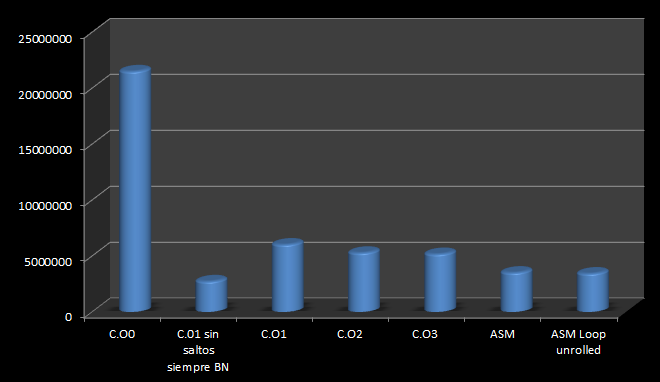
\includegraphics[scale=1]{imagenes/fcolor-grafico.png} 

\par
\bigskip
Una prueba adicional se hizo mientras se corria paralelamente un programa que utilizaba el 100\% del cpu arrojo resultados proporcionales. A continuacion de presentan en un grafico las relaciones entre las mediciones en estado $idle$ y en estado $100\%$ load.\\

\begin{center}
    \begin{tabular}{|l|l|l|l|l|l|}
        \hline
        Medición  & C.O0  & C.O1 & C.O2  & C.O3  & ASM LU  \\
        \hline
        Load & 33009164& 10239740  &7165908& 6709664 &4677277 \\
        \hline
        Idle & 21499106 & 6018971 & 5282602 & 5169947 & 3426934 \\
        \hline
        Relacion de incremento & 53\% & 70\% & 35\% & 30\% & 30\% \\
        \hline
    \end{tabular}
\end{center}
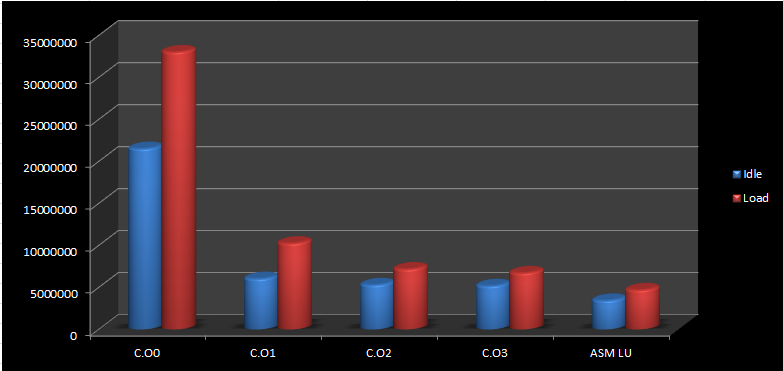
\includegraphics[scale=0.85]{imagenes/fcolor-grafico2.png} 

\subsubsection{Diferencias estructurales de las diferentes versiones analizadas}

En esta seccion nos centraremos en analizar las diferencias entre la version SIMD y las versiones C con sus diferentes niveles de optimizacion, de esta forma esperamos poder explicar los resultados numericos de la seccion anterior.
\\
\\
\textbf{Consideraciones iniciales:}\\
\par
Notoriamente entre la version del algoritmo en C y la version del algoritmo utilizando SIMD lo primero que hay que ver es que en la version de C se lee y procesa un pixel de origen por ciclo, mientas que utilizando SIMD, se procesan paralelamente 4 pixeles en instrucciones atomicas. Asi tambien cambia la forma de pensar el algoritmo como una division en casos con saltos condicionales entre ramificaciones de la ejecucion, hacia un pensamiento mas enfocado en procesamiento paralelo de valores, en los cuales mediante mascaras decidimos cuales componentes se procesaran con cada caso del filtro y luego, al ser casos disjuntos, pueden ser mezclados y escritos a destino, luego de realizar las conversiones y/o mezclados necesarios. 
\\
\textbf{Aclaracion sobre multiplicidad:} No tuvimos en cuenta los casos en donde la entrada tuviera un tamaño en pixeles que no fuera un multiplo de 4. Asumimos esta precondicion sobre la entrada para simplificar el algoritmo, podria solucionarse de forma sencilla sobre el codigo realizado, realizando un calculo de resto modulo 12 y una resta al puntero indice fuera del ciclo. Para informacion mas detallada de como solucionar este problema, dirigirse a la seccion del filtro \textbf{decode} donde se explica con mas detalle.
\\
\\
\textbf{Desensamblado de la implementacion original en C}\\
\par
Tomemos el codigo desensamblado con la herramienta \textbf{$objdump$} y busquemos posibles optimizaciones.
Podemos observar en el desensamblado del C sin optimizaciones, que las variables locales se utilizan como espacio de pila, produciendo un acceso a memoria cuando son requeridas para leer o escribir.Tambien afecta el traslado adicional entre memoria y registros para realizar operaciones.
\begin{center}
  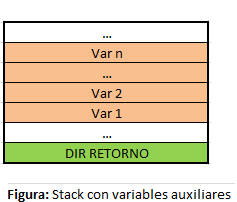
\includegraphics[scale=1]{imagenes/var-stack.png} 
\end{center}

Se encontro tambien la optimizacion en la division por 3 con el metodo de fraccion con denominador potencia de 2 mencionado anteriormente.

El resto del codigo parece acorde a la implementacion en C, de hecho es asi para permitir una correcta depuracion segun la documentacion de $GCC$.\\

Obviamente, el hecho de acceder a memoria para las variables locales, mas alla de lo que mejore la memoria cache, puede ser optimizado utilizando los registros internos del CPU y evitar estos accesos.\\
\\
\textbf{Incrementando la intensidad de la optimizacion: Primer nivel de optimizacion O1 }\\

En este modo se puede observar claramente el aprovechamiento de los registros internos del cpu para almacenar valores y variables temporales y evitar los accesos a memoria innecesarios. Asi tambien se observa que cambio el modo de direccionar la matriz ahora de una forma mas directa y con menor cantidad de instrucciones.

Es notorio el cambio en el tiempo de ejecucion este cambio, basta ver los graficos para ver que la reduccion considerable de accesos a memoria produjo una mejora importante.
\\
\\
\textbf{Analizando las optimizaciones mas agresivas:} O2 y O3\\
\par
$GCC$ nos ofrece una amplia variedad de flags para optimizar, se puede especificar en particular cada una de las posibles optimizaciones a realizar al codigo para obtener un ajuste fino. Por motivos de tiempo, solo analizaremos los flags que permiten optimizar de una forma automatica con cierto grado de agresividad, cada uno de estos flags engloba un grupo de optimizaciones particulares al codigo.
\\
\\
Un breve listado de las posibles optimizaciones estandares se muestra debajo:\\

\begin{center}
    \begin{tabular}{|l|l|}
        \hline
          Intensidad  & Descripcion\\
          \hline
          O0  & Casi ninguna transformacion al codigo, solo pasaje a assembler.  \\
          \hline
          O1  & Optimizaciones que no consuman mucho tiempo de compilacion.   \\
          \hline
          O2  & Optimizaciones que modifican el orden de ejecucion mejorando \\
           &  la velocidad del codigo resultante. Pueden verse alteradas variables \\
           &  del usuario y el cuerpo de algunas funciones.   \\
          \hline
          O3  & Optimizaciones que modifican aun mas el orden de ejecucion y pueden o no mejorar  \\
           &  la velocidad del codigo resultante. Puede verse alterada la semantica de las operaciones \\
           &  (particularmente las de punto flotante).\\
        \hline
    \end{tabular}
\end{center}

Existen otros parametros, entre ellos a saber $-Ofast$ que provee una mayor optimizacion que $-O3$ pero con el costo de no respetar los estandares. Por ejemplo, se implementa la optimizacion $ffast-math$ que acorde a la documentacion de $GCC$ puede producir errores en donde se espere una implementacion exacta del estandar IEEE o ISO de las funciones matematicas, es decir, puede verse alterada la precision de ciertos calculos.\\

Otro modo de optimizacion es $-Os$ que optimiza el tamaño del codigo manteniendo las optimizaciones de $-O2$ que no interfieran con el objetivo de este modo.\\

\textbf{Nota:} Para mas informacion dirigirse a:\\
\\
  \url{http://gcc.gnu.org/onlinedocs/gcc/Optimize-Options.html}\\
  \url{http://www.redhat.com/magazine/011sep05/features/gcc/}\\
\\

\subsubsection{Conclusiones acerca de las mediciones}
Luego de realizar estos analisis, podemos concluir acerca de las optimizaciones brindadas por el compilador $GCC$ que mejoran sorprendentemente la performance del mismo algoritmo, el mayor salto en rendimiento se ve con el primer nivel de optimizacion $O1$ que brinda el compilador. Asi mismo, la implementacion en assembler con SIMD obtiene mejores resultados que el C optimizado en su maximo nivel. El desenrrollado de ciclos brindo alguna mejora adicional, pero no demasiado significativa, y finalmente con respecto a los saltos condicionales, es muy notorio, como el procesador con su prediccion de saltos puede acelerar muchisimo la ejecucion, menos de la mitad de ciclos, ejecutando siempre la rama de ejecucion con mas costo, en este caso pasando siempre a blanco y negro realizando calculos aritmeticos de punto flotante, creemos que esto se debe a que la cpu no puede predecir cosas sobre los datos, condicion por la cual se evalua la guarda del salto condicional eliminado para el experimento.\\

Con respecto a los experimentos realizados con otra aplicacion utilizando el $100\%$ del cpu, se debieron correr 2 aplicaciones paralelamente que consuman el total del cpu, pues con una sola, creemos que al ser multicore, trasladaba el procesamiento a un solo core, dejando equilibrado el sistema operativo sobre los cores restantes. Los resultados fueron proporcionales, con excepcion de la version sin optimizaciones de C, atribuimos este valor atipico, a la cantidad de accesos a memoria que realiza esta version con respecto a las demas testeadas.
\\
Como objetivo de este tp, logramos comprobar la efectividad de las instrucciones SIMD a la hora de realizar calculos identicos a varios datos que pueden paralelizarse.

\subsubsection{Aclaraciones especiales respecto a los tests del fcolor}
Hay un test particular \textbf{test-fcolor-city.tar.gz} que tiene desactualizado el threshold en la pagina de la materia. Remitirse al email enviado por Marco Vanotti en la fecha 20-09-2013 en el cual explica como alterar el threshold del comando, cambiando su valor de 5000 a 71. Luego de este cambio, nuestro algoritmo pasa dicho test.
\newpage


\subsection{Miniatura}

\par
\bigskip
El filtro miniatura busca crear un efecto de miniaturizacion de una seccion de una imagen. Esto se logra mediante la aplicacion de un filtro de blureado de pixeles a una banda superior e inferior de la imagen, creando de esta forma en la banda central un efecto de miniatura. 

El filtro de blureado se basa en la aplicacion de una matriz de coeficientes a los pixeles circundantes al pixel objetivo y el cambio de los valores de color del mismo por el promedio de los resultados de las multiplicaciones, siendo los coeficientes representantes a una campana de gauss, se logra el disfuminado del pixel objetivo. Para maximizar el efecto, se pasa repetidas veces el filtro sobre la imageen, reduciendo la caantidad de filas por banda, creando asi un blureado en degrade haia el centro de la imagen.
\\
Para la implementacion del filtro para el trabajo se utiliza una matriz de dimension 5, con lo cual, por la simetria de la campana, se poseen 25 valores de los cuales solo 6 son distintos entre si. Al aplicarse esta matriz se debe considerar que, al posicionarse el pixel objetivo en el centro de la misma, se debe contar con pixeles en el radio de la matriz, para poder aplicarse los coeficientes. Debido a esto, se toman 2 pixeeles de marco para la imagen en los bordes, los cuales quedaran iguales.
\\
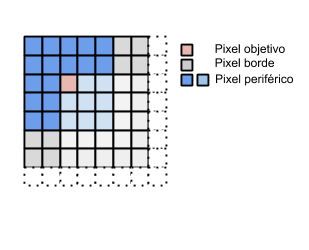
\includegraphics[scale=1]{imagenes/bordes-matriz-super.png} 

Los coeficientes de la matriz, siendo valores comprendidos entre 0 y 1, requeririan la utilizacion de valores de punto flotante. Al ser las operaciones con los mismos mas caras en tiempo, se pasan los numeros a valores enteros, multiplicando los flotantes por 100. La presicion del resultado se conserva porque los coeficientes son de presicion centesimal.
\\
Para no aumentar el brillo de la imagen se divide por la suma de todos los coeficientes de la matriz (6) .A esto se le agrega la division por 100 para generar los valores correctos.


\subsubsection{Descripcion del algoritmo}
\par
\bigskip
Para la descripcion del algoritmo contamos con el pseudocodigo acotado de la solucion implementada, el cual servira de guia para la interpretacion de las tareas realizadas. La logica del mismo 
fue pensada para tamaños de imagenes a partir de 5 x 5 pixeles en el caso de C y  5 x 7 en el caso de assembler. Para explicar el algoritmo se describira en primera instancia la idea y consideraciones generales que comparten ambas versiones; para luego profundizar en cada una, detallando en la seccion de assembler, los cambios realizados para la adaptacion a las instrucciones SIMD.
\par
\bigskip
\lstinputlisting[language=C,tabsize=4, numbers=left, numberstyle=\tiny\color{black},mathescape=true, backgroundcolor=\color{gray}, rulecolor=\color{black}, keywordstyle=\color{blue}, commentstyle=\color{dkgreen},stringstyle=\color{mauve}, numbersep=5pt, basicstyle=\scriptsize]{fuentes/pseudominiature_filter_c.c}

\begin{enumerate}
\item \textbf{La matriz de coeficientes} \\
La matriz, como fue dicho en la introduccion, al ser simetrica posee solo 6 valores distintos entre si: 0.01, 0.5, 0.18, 0.32, 0.64 y 1. Estos valores son guardados en forma entera multiplicandolos por 100, sin perder presicion.\\

\item \textbf{Recorrido de la imagen} \\
En una primera implementacion se recorria la matriz de pixeles en forma lineal (tomando la matriz como una lista). No obstante se vio que la lectura y desarrollo del codigo se complicaba a la hora de calcular limites y casos bordes, al contrario de un recorrido por filas y columnas.\\

\item \textbf{Posicion del pixel en la matriz} \\
Al hacerse un recorrido por filas y columnas es necesario un calculo adicional para traducir la posicion: por lo que la posicion se calcula haciendo columna * tamPixel + fila * width * tamPixel, siendo tamPixel = 3 (imagen en RGB).\\

\item \textbf{Limites de bandas e iteraciones} \\
Los limites de las bandas por iteracion fueron dados por consigna mediante la aplicacion de una ecuacion que presenta una division. No estaba especificado lo que se debia hacer en caso de que la misma no fuese exacta (con resto). Se pudo determinar en la etapa de testeo, que en el caso de la bada superior, se debia redondear para arriba. Este cambio se realizo al notar que solo el ultimo test: test-miniature-03-08-5-city; aparecian en el primer frame procesado, en la banda superior, una diferencia en las imagenes por 2 pixeles. Al aumentar la cantidad de iteraciones del test y bajar la tolerancia en la comparacion, se pudo determinar que en las bandas de las iteraciones de division no exacta, se perdia una linea de pixeles. El cambio permitio pasar 29 frames del test final.
 Otros pxeles fueron marcados como diferentes en la esquina inferior del frame 30. Se intento la aplicacion de la misma solucion que para el caso anterior pero sin exito. Al ser los ultimos pixeles filtrados de la imagen (5 pixeles diferentes), y ser objetivo de varias iteraciones, se supuso  algun tipo de error numerico entre nuestra version y la version que produjo las imagenes del test. Se descarto la posibilidad de perdida de presicion ya que en las operaciones para adaptar los coeficientes a valores enteros, no se recorto ninguna cifra y en las operaciones se cuido de no producir redondeos de mas.
\\

\item \textbf{Bordes de la imagen} \\
El algoritmo solo se puede aplicara a los pixeles cuya posicion diste en 2 de los bordes de la imagen. No obstante, en la etapa de testeo se determino que, para pasar exitosamente los tests, se debia considerar los pixeles a partir de la fila 4\\

\item \textbf{Intercambio} \\
Para aumentar el efecto del blureado se pasa la imagen blureada a la proxima iteracion como imagen fuente.\\

\end{enumerate}

Hasta este punto el algoritmo implementado en C y en Assembler son iguales. La diferencia entre ellos radica en la implementacion de \textbf{aplicarFiltro} y \textbf{copiarIgual}\\

\subsubsection{Implementacion en C}

Tanto en la aplicacion del filtro como en la copia de los pixeles se hace un procesamiento por pixel, es decir, se lee un pixel se copia un pixel.Como para cada pixel a filtrar son necesarios 2 filas de pixeles circundantes, la imagen mas chica a evaluar debera tener por lo menos una dimension de 5 x 5 pixeles.

\lstinputlisting[language=C,tabsize=4, numbers=left, numberstyle=\tiny\color{black},mathescape=true, backgroundcolor=\color{gray}, rulecolor=\color{black}, keywordstyle=\color{blue}, commentstyle=\color{dkgreen},stringstyle=\color{mauve}, numbersep=5pt, basicstyle=\scriptsize]{fuentes/pseudo-filtro-mini.c}

\par
\bigskip
El filtro obtiene un cuadrado de pixeles de 5 x 5 tomando como centro el pixel a blurear y a cada pixel, dependiendo su posicion se lo multiplica con un coeficiente de la matriz. El resultado se guarda en una variable temporal por cada color del pixel. Al finalizar de multiplicar a todos los pixeles del cuadrado, normalizamos por 600 (6 del brillo y 100 por la conversion a enteros).

Este procedimiento se realiza 25 veces, que es la cantidad de pixeles dentro del cuadrado. Finalmente se escribe el pixel objetivo en el archivo de destino.

\subsubsection{Implementacion en assembler utilizando set de instrucciones SIMD}

Al disponer de instrucciones que nos permiten paralelizar calculos, se busco la forma de juntar el procesamiento de las partes del algoritmo en donde se analizaba de a un dato. Este aspecto es fundamental, ya que nos permite disminuir los accesos a memoria, principal cuello de botella de C. La idea implementada con SIMD se dividio en 2 aspectos del algoritmo: la copia de pixeles iguales, como los bordes y el frame central, y el filtrado de aquellos pixeles de las bandas superior e inferior. Incluido en la optimizacion de accesos a memoria, se busco, aparte del copiado de mas de un pixel a la vez, optimizar los calculos con la matriz, dado que representa el grueso de peticiones a memoria de nuestra solucion.

Al estar trabajando con mas de un dato, surgieron casos bordes y detalles que en C, no habia. En los siguientes puntos se muestran los distintos aspectos que fueron adaptados para el uso de las SIMD.

\textbf{Copia de pixeles:}

Para la copia de pixeles iguales se aprovecho el hecho de que los pixeles levantados son consecutivos, por lo que se pudo copiar de a 5 pixeles enteros por acceso a memoria. Esto se debe al uso de los registros de 16 bytes, (descartandose el ultimo byte).

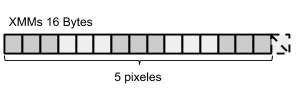
\includegraphics[scale=0.7]{imagenes/xmm-pixeles.png} 
\\
\textbf{Caso borde:}
\\
Bajo este modo de copia surge un caso borde al final del archivo de imagen. Como se esta levantando de a 16 bytes, el archivo puede no ser divisible por dicho numero (en la mayoria de los casos), con lo cual se debe detectar la proximidad al final del archivo y correr el puntero de la memoria a levantar 16 bytes antes del borde.

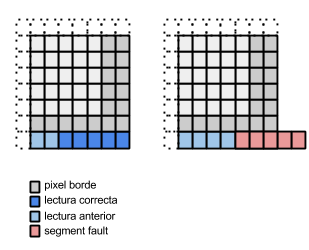
\includegraphics[scale=0.7]{imagenes/caso-borde-5.png} 

\textbf{Filtro:}
\\
Para la implementacion del filtro en Assembler se realizaron 2 etapas: Paralelismo en cuanto a calculo con la matriz de coeficentes y paralelismo en cuanto a pixeles copiados.
\par
\bigskip
La primera etapa busco reducir el numero de accesos de memoria para el calculo del producto de los coeficientes de la matriz con los pixeles circundantes al objetivo. Se aprovecho el hecho de que la longitud de las filas de la matriz y la cantidad de pixeles levantados por XMMs coincidian, con lo cual se procedio a calcular el resultado parcial de los productos y sumas de cada fila. Luego se normalizaba con 600 y se pasaba el valor del pixel a memoria:

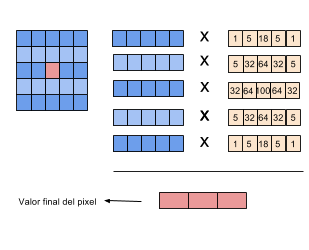
\includegraphics[scale=0.7]{imagenes/version1-miniature.png} 

De esta forma estariamos levantando de memoria 5 veces por cada pixel evaluado, con lo que reduce los 25 accesos por pixel de la version en C.

La segunda tapa fue la de lograr incorporar mayor cantidad de pixeles al resultado. Por razones de cantidad de registros se logro procesar un maximo de 3 pixeles a la vez. Esto se alcanza mediante el solapamiento de cuadrados de 5 x 5 de los 3 pixeles:

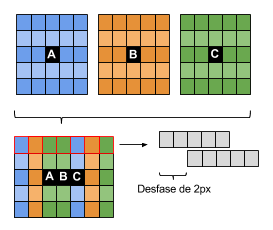
\includegraphics[scale=0.7]{imagenes/solapamiento-cuadros.png}  Filtro miniature: Imagen de solapamiento de datos y aprovecahmiento de xmms

De esta forma se estarian efectuando 10 accesos a memoria por cada 3 pixeles evaluados. En cuanto el archivo de entrada debera contar ahora con 2 columnas mas, aumentando a 5 x 7 la menor imagen filtrable por el algoritmo
\\
\textbf{Caso borde:}
\\
Al igual que en la copia de pixeles, el filtrado posee un caso borde en la ultima fila que puede ser filtrada: la antepenultima. Como para el procesamiento del pixel son necesarias las dos filas inferiores al pixel y las dos columnas del borde, si no se detecta a tiempo se produce un error de acceso a segmento. Esto se evita añadiendo logica de borde la cual, de estar analizando alguna de los ultimos 3 pixeles filtrables, se tome el puntero de memoria a levantar de forma que en el calculo de levantado de las filas para los coeficientes, no nos genere un error de segmento:\\

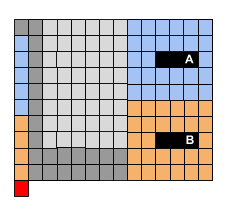
\includegraphics[scale=0.7]{imagenes/caso-borde-filtrar.png} 

En la imagen anterior, se pueden ver dos situaciones. El cuadro de pixeles donde se encuentra el pixel A, llego a un borde y lee datos basura del otro borde de la matriz. Sin embargo esto no presenta ningun problema, ya que, los pixeles leidos existen y el dato erroneo del pixel A que se guarda en la nueva imagen, sera pisado cuando el algoritmo detecte en una iteracion siguiente de que pertenece al borde (explicado en seccion siguiente), por lo que copiara nuevamente a la posicion de destino el valor correcto.

En el caso B se puede ver que se ha llegado al final de la imagen, por lo que, al contrario del caso A, si leo un pixel del borde, no va a ver una fila inferior para leer, con lo que nos iriamos del segmento. Para contrarrestar esto, la logica de borde analiza que de estar en la antepenultima fila filtrando y si estamos en el antepenultimo pixel que se debe filtrar, levante y procese los 3 pixeles, se saltee directamente los 2 proximos pixeles (ultimo y anteultimo, porque de no saltearlos en la proxima iteracion volveriamos al caso borde creanso un loop infinito) y adelante el cursor de columna directamente a los pixeles del borde.


\textbf{Solapamiento entre filtrado y copiado:}
\\
Al estar analizando de mas de un pixel a la vez, se da la situacion en que: por ejemplo, al levantar 5 pixeles para copiar y dejar igual, estemos levantando uno o varios que deben ser filtrados, con lo cual de pasar a analizar los proximos pixeles, estariamos produciendo una imagen con error. 

Para evitar esto estamos obligados a analizar indice de pixel a indice, determinando en cada caso cuando debemos filtrar y cuando no. Para seguir con la idea del procesamiento de 3 pixeles (o 5 en el caso de copia sin modificacion) establecemos un contador el cual no indica cuantos pixeles fueron analizados previamente. Si al analizar un pixel el contador no esta en cero, entonces podemos evitar la lectura de memoria de ese pixel. Al estar escasos de registros de proposito general, se utilizo un solo registro para llevar el contador de ambos: el mismo toma valores de 0 a 5 en caso del levantamiento por copia, y de 6 a 8 para los filtrables: 

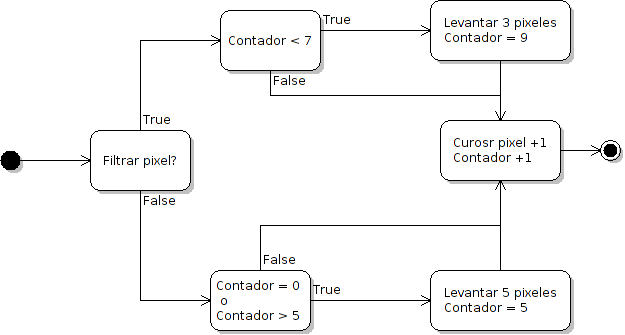
\includegraphics[scale=0.5]{imagenes/uml-mini.png}



\subsubsection{Detalle de procesamiento de filtrado de a 3 pixeles}

Suponiendo a los pixeles A, B, C, pixeles a ser filtrados, vamos a detallar el calculo de los colores. Para el procesamiento se va a necesitar un rectangulo de pixeles que contendra toda la informacion que necesitamos evaluar para el resultado final. Cada fila de este rectangulo se puede obtener mediante 2 accesos de memoria, como puede verse en la imagen anterior de solapamiento de datos.\\

Los datos obtenidos en estos 2 registros son utiles para el calculo de cada uno de los 3 pixeles, siendo utiles para mas de uno a la vez, con lo cual, se los debe multiplicar por mas de un coeficiente distinto.

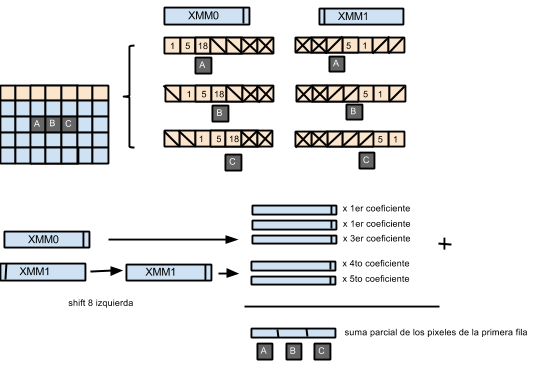
\includegraphics[scale=0.8]{imagenes/mini-matriz-descomposicion.png}

Como cada resultado de cada coeficiente le es util de forma ordenada a cada pixel objetivo de forma vertical, se puede aprovechar su uso para un procesamiento en paralelo. Como puede verse en la imagen anterior, en el caso del coeficiente 1 en el XMM0, multiplica el primer, segundo y tercer pixel. Usando esto, podemos multiplicar directamente a todos los pixeles de la fila (osea a cada color) por el coeficiente y sumarselo a las sumas parciales de cada uno de los 3 pixeles objetivo (ya que estamos usando solo 3 pixeles en cada levantada del XMM0 y XMM1).

En el caso del primer coeficiente, los pixeles quedan justo alineados para sumar al resultado parcial. Esto no ocurre para los demas, estando para el segundo coeficiente desfasados en un pixel y para el tercero en 2. Para el 4to y quinto los pixeles se recuperan en un segundo XMM, el cual tiene un corrimiento de 1 pixel y 2/3 para levantar de memoria. Se hace de esta forma, con 1/3 (8 bits) de pixel anterior leido al principio para que todo lo levantado por los XMM sean datos validos y a usar en los calculos del filtro. Este corrimiento de 1/3 se  compensa corriendo los datos del XMM 8 bits, ya que es un dato que ya se uso para los coeficientes anteriores, y no es necesario para los calculos del 4to y 5to, puede ser ignorado.

Al finalizar la multiplicacion por cada coeficiente (cuyo resultado esta en las primeras 3 posiciones del XMM) solo falta la suma con las sumas parciales guardadas anteriormente y luego pasar a la segunda fila. Para cada fila la logica del procedimiento es equivalente. En lo unico que varia es el los coeficientes de cada posicion y en el corrimiento por fila para levantar los datos de la matriz.

Al finalizar el procesamiento de los pixeles debemos dividir por el coeficiente normalizador (6) y el ajuste por considerar integer a los coeficientes de la matriz (100) y finalizar ordenando los pixeles obtenidos para escribirlos en memoria.\\


Para hacer estas multiplicaciones, sumas y divisiones en paralelo se tuvo que tener en cuenta la perdida de presicion de datos. Dado que cada color esta representado en 8 bits, al multiplicarlo por un valor entero se corre el riesgo de un overflow. El maximo numero posible con los coeficientes de la matriz estaria representado por el color 255 y el coeficiente 1 (osea 100) con lo cual tendrriamos al 25500 como supremo y maximo del conjunto, que entra en un tamaño de word.\\



Para la suma de cada colr esta sumando el valor de 25 words con un valor maximo de 25500 con lo cual se tendria como nueva cota a 637500, el cual entra en un tamaño de doubleword. Por esta razon, la suma total de cada pixel estaria representada por 3 doublewords, con lo cual el resultado de los 3 pixeles entra en 3 XMM, teniendo en el ultimo de ellos solo la primera doubleword con datos de color.\\

La operacion de desempaquetamiento se hace en otro orden, respetando la misma idea: primero se descomprimenl los 8 bits de cada color a word. Ahora se usa la operacion PMULLW y PMULLHW, las cuales hacen una multiplicacion de a word y devuelven un doubleword.. que seria exactamente lo que se necesita en este caso, ahorrandosse un paso de desempaquetamiento:\\


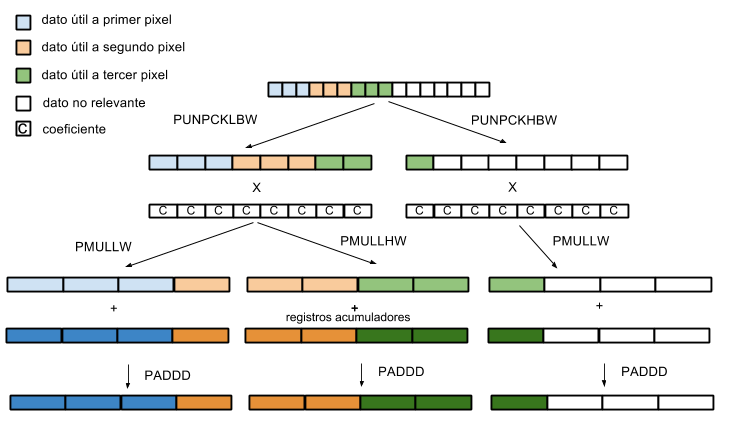
\includegraphics[scale=0.5]{imagenes/operaciones-xmms-fila.png}




El siguiente paso es convertir estos 3 registros de double words en 1 de 16 bytes en donde los colores esten en orden, al igual que los pixeles para asi poder pasarlos de una a memoria.

Para esto primero vamos a normalizar el resultado por 600. Como se busca hacerlo en paralelo, genero un registro con 600 repetido en cada double word y divido de forma paralela. Para ello necesito pasar antes a punto flotante para poder usar las funciones SIMD, y luego retornar los valores a enteros. Con la operacion DIVPS pasamos a dividir los floats por floats empaquetados, luego con la operacion CVTDQ2PS recuperamos el resultado de las divisiones con redondeo por truncamiento a doubleword integers.


Teniendo ya los resultados finales, lo que falta es la reconversion a 8 bit de cada color.
Para los 2 primeros registros de resultados podemos empaquetar ambos registros a word con una sola instruccion (PACKSSDW) y de word a byte con otra (PACKUSWB):\\

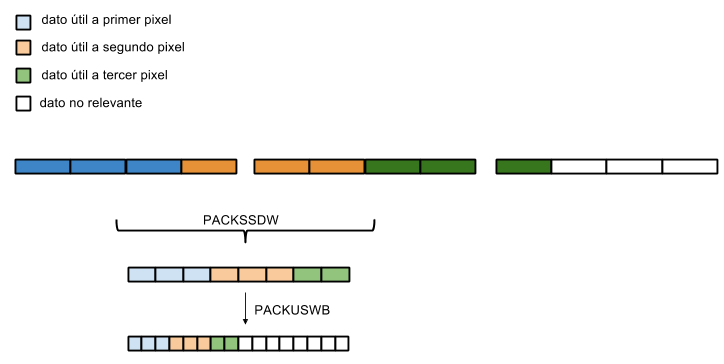
\includegraphics[scale=0.5]{imagenes/empaquetamiento.png}

Como se puede ver en la imagen anterior, aun queda un color del ultimo pixel en el ultimo registro, con lo cual debemos insertarlo en el registro de retorno para poder guardarlo en memoria.

Para lograr esto vamos a hacer uso de una mascara que nos aislara el color en la posicion en la cual tengamos que insertarlo en el registro destino. El valor a aislar, aunque sea double word, vale notar que su valor no supera a 255, ya que posee el valor de un color valido, por lo que el numeo en integer ocupa el tamaño de 8 bits. Gracias a esto se lo puede considerar tambien como un word integer y usar la instruccion PINSRW para insertar en el lugar indicado del registro el valor. Al registro destino se le setearan los bits en 0 en el lugar donde tengamos que insertar el valor resagado y mediante una suma logica vamos a pegar el color en el lugar correspondiente. Al entrar en un byte el valor pegado, los ceros de la parte alta del word no cambian los valores anteriormente empaquetados.\\

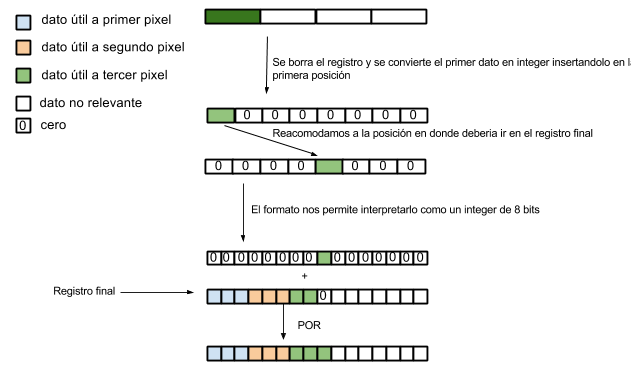
\includegraphics[scale=0.5]{imagenes/reacomodamiento.png}

\subsubsection{C vs Assembler con SIMD}

Las diferencias mas fuertes en la estructura del algoritmo en las implementaciones pueden reducirse a 2, y dejar las demas como consecuencias de estas: La cantidad de datos procesados y accesos a memoria. Como se explico anteriormente, la resolucion en C debe hacer 25 accesos a memoria por pixel filtrado y un acceso por pixel copiado (el que lo pasamos directo). Por otro lado, el algoritmo de assembler logra reducir los accesos a 10 por cada 3 pixeles evaluados, gracias al solapamiento de los cuadros de pixeles y la capacidad de los registros XMM de obtener de a tandas de 5 pixeles. Por esto tambien se pudo reducir los accesos para dejar pixeles iguales, copiando de a 5 pixeles por vez, la velocidad del algoritmo aumenta drasticamente por la manipulacion en paralelo de estos datos que no necesitan procesamiento alguno. Los resultados pueden ser vistos en los siguientes graficos que comparan la cantidad de ciclos consumidos por el CPU para 2 archivos distintos corridos sobre C y sobre assembler:


\subsubsection{Tiempos de ejecucion de diferentes experimentos}

\par
\bigskip
\textbf{Caracterizacion del experimento: }
\begin{itemize}
    \item \textbf{Iteraciones: } 5
    \item \textbf{Comando C City: }  ./tp2 -t 5 miniature -i c city.avi 0.3 0.8 3
    \item \textbf{Comando ASM City: }  ./tp2 -t 5 miniature -i asm city.avi 0.3 0.8 3
    \item \textbf{Comando C Ink}./tp2 -t 5 miniature -i c ink.avi 0.3 0.8 3
    \item \textbf{Comando Asm Ink}./tp2 -t 5 miniature -i asm ink.avi 0.3 0.8 3
\end{itemize}
\par

\textbf{Resultados:}\\
\begin{center}
    \begin{tabular}{|l|l|l|l|l|}
        \hline
        Medición  & C ink.avi  & ASM ink.avi & C city.avi  & ASM city.avi \\
        \hline
        Ciclos por llamada	&	459987456	& 76210288 & 459888288 & 76193352 \\
        \hline
    \end{tabular}
\end{center}
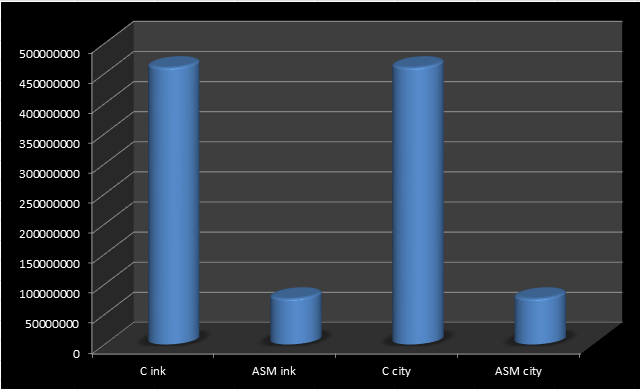
\includegraphics[scale=1]{imagenes/miniature-grafico.png} 

\subsubsection{Comentarios sobre los resultados obtenidos del experimento}

Las diferencias impactan notablemente sobre los tiempos de ejecucion del algoritmo aumentando notoriamente la velocidad de procesamiento de los videos objetivos en un \%600. De esta forma se puede concluir que a la hora del procesamiento de archivos de medios, las instrucciones SIMD logran un mejor aprovechamiento del poder de computo del CPU al permitirnos manipular mayor cantidad de datos y de forma paralela sobre memoria disminuyendo los accesos a ella.

\newpage

\subsection{Decode}

El filtro decode consiste en la decodificacion de un texto embebido en los bits menos significativos de los pixeles de una imagen. Cada 4 bytes, se toman los dos bits menos significativos de cada uno y se obtiene un nuevo byte que es la codificacion ascii de un caracter del texto. Tambien se utilizan el tercer y cuarto bit menos significativo de cada byte para saber como interpretar esos bits y aplicarles operaciones.
\par
\bigskip
Se implemento una primera version del algoritmo en C, analicemos el algoritmo y luego veamos que optimizaciones se le aplicaron.
\subsubsection{Descripcion del algoritmo}

\textbf{Nota: la idea de este codigo es entender como funciona nuestro algoritmo, por ello se eliminaron varias partes del codigo original.}\\
\lstinputlisting[language=C,tabsize=4, numbers=left, numberstyle=\tiny\color{black},mathescape=true, backgroundcolor=\color{gray}, rulecolor=\color{black}, keywordstyle=\color{blue}, commentstyle=\color{dkgreen},stringstyle=\color{mauve}, numbersep=5pt, basicstyle=\scriptsize]{fuentes/pseudodecode_c.c}
\textbf{Explicacion del algoritmo:}\\
Analicemos por partes que hace este algoritmo:\\
\begin{itemize}
    \item \textbf{Lectura de 4 bytes de origen:} Lineas 4-7\\
        En esta sección se leen de origen 4 bytes que contendrán en los 4 bits menos significativos de cada uno la informacion correspondiente a un char del mensaje codificado.
    \item \textbf{Filtrado con mascaras de valores relevantes:} Lineas 10-19\\
        Luego, debemos separar de alguna manera los bits que nos interesan del resto, para ello utilizamos mascaras de bits que por medio de operaciones logicas de conjuncion y corrimiento nos permiten quedarnos con los bits que nos interesan, en este caso code(primeros 2 bits) y op(tercer y cuatro bit).
    \item \textbf{Procesado del code segun el op:} Lineas 22-25\\
        Ya tenemos organizados los datos de las etapas anteriores de forma tal que podemos aplicar una serie de comparaciones al op para saber cual operacion realizarle al code correspondiente, para esto utilizamos una funcion auxiliar que nos devuelve el code listo para ser combinado.
    \item \textbf{Combinacion y escritura a destino:} Lineas 28-30\\
        Tal como dice el enunciado, realizamos un mezclado de los 4 bytes(notar que solo se utilizan 2 bits de cada uno) por medio de corrimientos y operaciones logicas de disyuncion. De esta forma hemos armado un caracter del mensaje, el cual es escrito al buffer de salida pasado por parametro.
\end{itemize}
\bigskip
\textbf{Optimizaciones realizadas:}
\begin{itemize}
    \item \textbf{Eliminacion de la llamada a la funcion auxiliar por medio de modificador inline:}\\
        De esta forma, con este modificador pretendemos eliminar los saltos de la llamada a funcion, requiriendole al compilador introducir el cuerpo de la funcion en cada invocacion a esta.
\end{itemize}

\bigskip
\textbf{Detalles de implementacion:}
\begin{itemize}
    \item \textbf{Multiplicidad de la cantidad de bytes a procesar:}\\
        En nuestra implementacion no tuvimos en cuenta el caso donde la cantidad de bytes a procesar no es multiplo de 16, es decir, que el ultimo ciclo, leeria memoria invalida al introducir una entrada que no respete esta precondicion de multiplicidad de tamaño.Para solucionarlo se podria implementar una solucion que consiste en iterar sobre los primeros k-bytes tal que k sea el primer multiplo de 16 hacia menos infinito. y luego, fuera de dicho ciclo, restarle al puntero 16 menos el resto modulo 16 del tamaño de la entrada y hacer un salto no condicional al comienzo del ciclo, luego de ejecutarse una vez mas, automaticamente la guarda se vuelve falsa y termina el ciclo.
\end{itemize}

\subsubsection{Implementacion en assembler utilizando set de instrucciones SIMD}

Luego de realizar la anterior implementacion en C, nos pusimos a pensar la mejor manera de utilizar SIMD con el set de instrucciones que teniamos a nuestro alcance.
Consideramos realizar la implementacion en assembler con la ventaja de poder utilizar los registros XMM de un tamaño de 16 bytes y maximizar su capacidad para leer mas de 4 bytes en cada ciclo. Dicho esto, la version en assembler obtiene 16 bytes por ciclo, y con las instrucciones de operatorias empaquetadas se espera procesar 4 veces mas datos por ciclo.\\
\\
\textbf{Nota: } En esta implementacion nos dimos cuenta que en muchos lugares utilizamos unicamente 2 bits de los 16 bytes empaquetados, pero dadas las instrucciones a nuestro alcance, consideramos que es la mejor implementacion en SIMD respetando un balance entre el set de instrucciones a nuestro alcance y el rendimiento.

\subsubsection{Analisis}
Antes de comenzar el ciclo principal nos vimos con la necesidad de declarar algunas mascaras como variables globales inicializadas para la manipulacion de los bits, y las cargamos en registros XMM para evitar esos accesos a memoria en cada iteracion de ciclo, que reducen significativamente la velocidad del programa. Estas mascaras son:

\par      
\bigskip
 \begin{figure}[!ht]
  \centering
     \begin{tikzpicture}
      \registroDieciseis{\xmm{14}}{0}{5}
       {3}{3}{3}{3} {3}{3}{3}{3}
       {3}{3}{3}{3} {3}{3}{3}{3}
  \end{tikzpicture}
  \caption{00000011 replicado, para hacer AND y filtrar los ultimos 2 bits}
\end{figure}

\par      
\bigskip
 \begin{figure}[!ht]
  \centering
     \begin{tikzpicture}
      \registroDieciseis{\xmm{15}}{0}{5}
       {12}{12}{12}{12} {12}{12}{12}{12}
       {12}{12}{12}{12} {12}{12}{12}{12}
  \end{tikzpicture}
  \caption{00001100 replicado, para hacer AND y filtrar el tercer y cuarto bit}
\end{figure}

\par      
\bigskip
 \begin{figure}[!ht]
  \centering
     \begin{tikzpicture}
      \registroDieciseis{\xmm{10}}{0}{5}
       {00}{00}{00}{00} {00}{00}{00}{00}
       {00}{00}{00}{00} {00}{00}{00}{00}
  \end{tikzpicture}
  \caption{para comparar los resultados y ver si es el op 0}
\end{figure}

\par      
\bigskip
 \begin{figure}[!ht]
  \centering
     \begin{tikzpicture}
      \registroDieciseis{\xmm{11}}{0}{5}
       {01}{01}{01}{01} {01}{01}{01}{01}
       {01}{01}{01}{01} {01}{01}{01}{01}
  \end{tikzpicture}
  \caption{para comparar los resultados y ver si es el op 1}
\end{figure}

\par      
\bigskip
 \begin{figure}[!ht]
  \centering
     \begin{tikzpicture}
      \registroDieciseis{\xmm{12}}{0}{5}
       {02}{02}{02}{02} {02}{02}{02}{02}
       {02}{02}{02}{02} {02}{02}{02}{02}
  \end{tikzpicture}
  \caption{para comparar los resultados y ver si es el op 2}
\end{figure}

\par      
\bigskip
 \begin{figure}[!ht]
  \centering
     \begin{tikzpicture}
      \registroDieciseis{\xmm{13}}{0}{5}
       {03}{03}{03}{03} {03}{03}{03}{03}
       {03}{03}{03}{03} {03}{03}{03}{03}
  \end{tikzpicture}
  \caption{para comparar los resultados y ver si es el op 3}
\end{figure}

\begin{itemize}
\item El primer paso es obtener los 16 bytes de la matriz mediante la operacion  MOVDQU XMM0, [RDI + R12] (donde RDI = src y r12 = index) y guardarlos en el registro \xmm{0}.

\end{itemize}

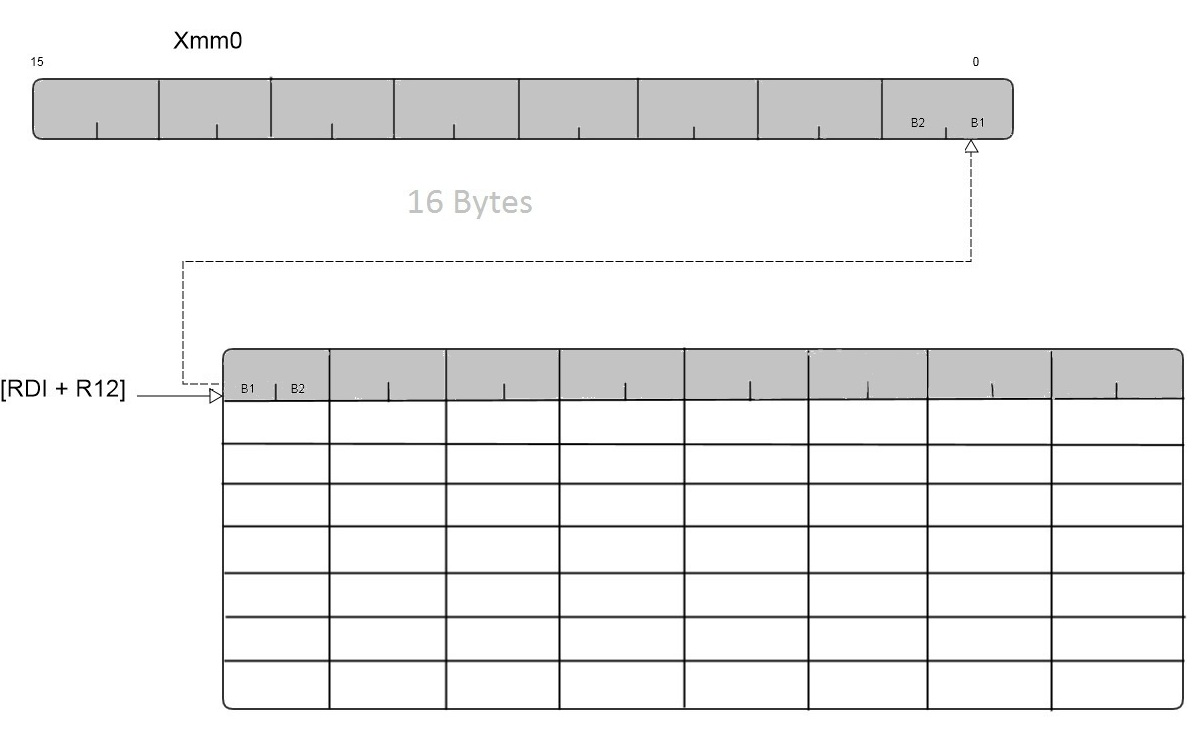
\includegraphics[height=10cm]{levantar.jpg} 

\begin{itemize}
\item Replicamos esos datos en \xmm{1}. Al hacer una operacion de conjuncion entre \xmm{1} con la mascara de \xmm{14} obtenemos los bits menos significativos de cada byte que son los codigos. Luego hacemos una nueva operacion de disyuncion logica entre \xmm{0} contra la mascara guardada en \xmm{15} y de esta forma nos quedan el tercer y cuarto bit de cada byte filtrado, que son la operacion a realizar sobre los codigos. Pero las operaciones nos quedan en el tercer y cuarto bit por eso utilizamos una intruccion de corrimiento PSRLQ para mover dos bits a la izquierda los datos obtenidos. De esta forma tenemos en \xmm{1} los codigos y en \xmm{0} los codigos de operaciones que nos dirán que modificacion realizar sobre ellos. 

Obtener codigos:

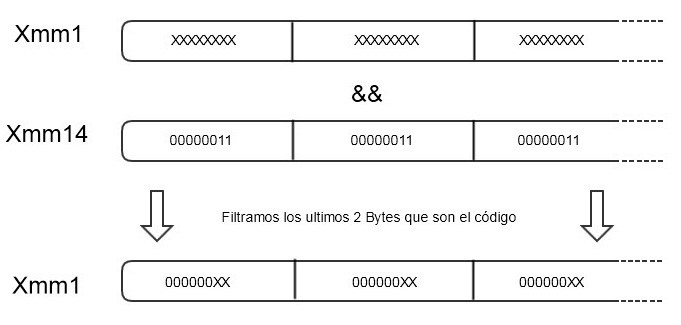
\includegraphics[height=7cm]{codigos.jpg} 

Obtener operaciones:

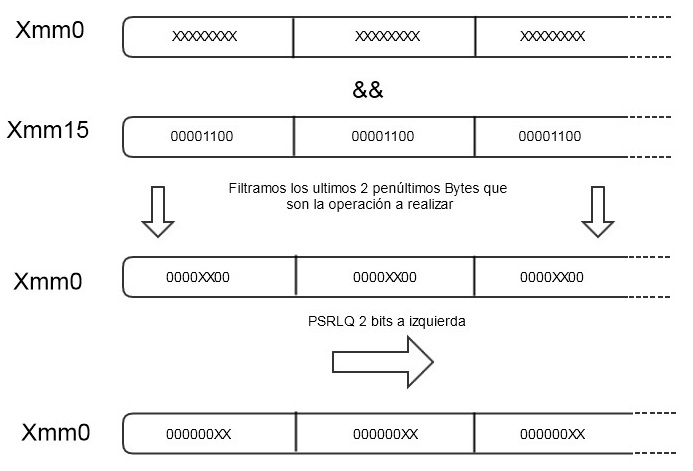
\includegraphics[height=10cm]{operaciones.jpg} 

\item Replicamos los codigos de operacion en \xmm{2}, \xmm{3} Y \xmm{4}. Paso seguido comparamos mediante la operacion PCMPEQB de comparacion empaquetada por igualdad cada registro \xmm{0}, \xmm{2}, \xmm{3} y \xmm{4} con las mascaras guardadas en los registros \xmm{10}, \xmm{11}, \xmm{12}, \xmm{13} respectivamente. Obtenemos en los registros el resultado de las comparaciones en forma de mascaras que contienen en cada posicion 0x00 y 0xFF dependiendo de si, para cada byte, en su posicion, estaba la operacion 0, 1, 2 o 3 originalmente en el registro comparado. ie. (\xmm{0} tiene 0XFF en las posiciones donde estaba la operacion 0, \xmm{2} tiene 0XFF en las posiciones donde estaba la operacion 1, etc.)

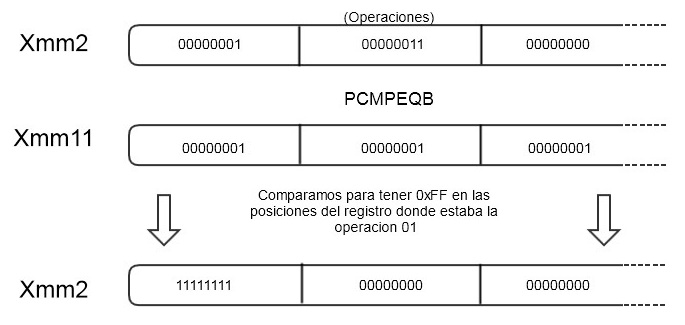
\includegraphics[height=7cm]{comparacion.jpg} 

\item En los registros \xmm{5}, \xmm{6}, \xmm{7} y \xmm{8} replico los codigos (anteriormente en \xmm{1}), y aplico a cada uno una de las operaciones a realizar sobre codigos denotadas por los codigos de operacion. Luego, para cada registro, dependiendo de la operacion que le aplique, le aplicamos una operacion logica de disyuncion contra la mascara correspondiente \xmm{0}, \xmm{2}, \xmm{3} y \xmm{4}) a los bytes en cuyo indice estaba esa operacion. De esta forma entre \xmm{5}, \xmm{6}, \xmm{7} y \xmm{8} me quedan todos los codigos con las operaciones correspondientes aplicadas y notar que los bytes empaquetados , no se superponen entre registros. De esta forma, con una conjuncion logica puedo juntar todos en un solo registro y tengo en \xmm{5} los 16 bytes que solo tienen los 2 bits mas bajos ya procesados por las operaciones.

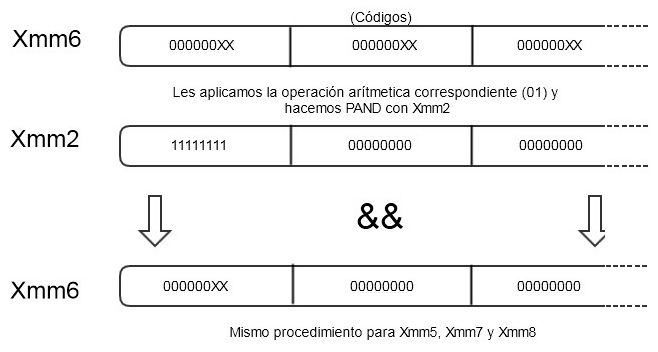
\includegraphics[height=7cm]{siguienteacomparaciones.jpg} 

Unimos resultados mediante POR's:

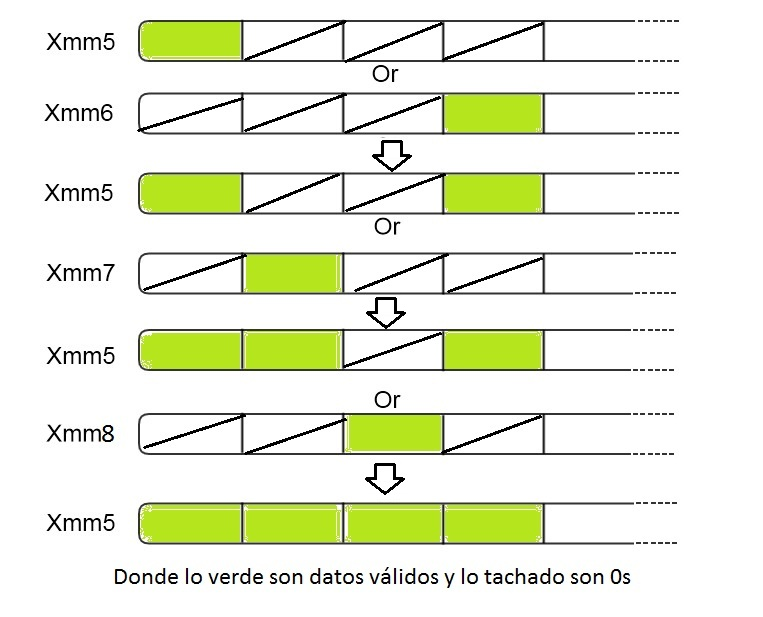
\includegraphics[height=8cm]{ors.jpg} 

\item Lo unico que queda pendiente es la combinacion de los codigos procesados para formar 4 caracteres ascii. Logramos esto mediante el uso repetido de la instruccion PEXTRB para extraer 4 bytes del registro \xmm{5}, copiarlos en \reg{8}, \reg{9}, \reg{10} y \reg{11},y realizar los corrimientos pertinentes a cada uno con el objetivo de acomodarlos en la posicion correcta y formar un byte entre todos aplicando una operacion logica de disyuncion. Esto se hace una vez por cada uno de los 4 caracteres, y la combinacion se almacena en los registros \texttt{AL}, \texttt{BL}, \texttt{CL}, \texttt{DL}

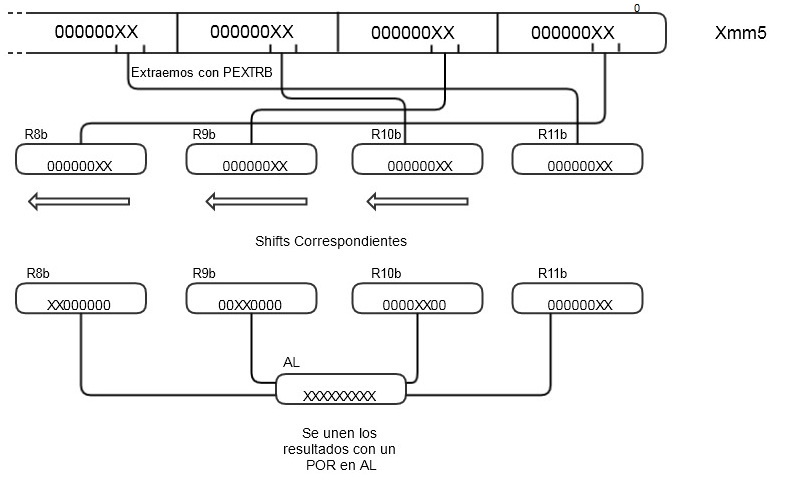
\includegraphics[height=9cm]{char.jpg} 

\item Finalmente copiamos los 4 bytes que contienen los 4 caracteres al buffer de salida. 

\end{itemize}

\subsubsection{Optimizaciones aplicadas al algoritmo}
\begin{itemize}
    \item \textbf{Implementacion de software pipelining - Ejecucion fuera de orden}
    Se implemento esta de la mejor forma a nuestro alcance tecnica para aprovechar la ejecucion fuera de orden que provee el cpu. Esto permite que instrucciones no $dependientes_{*1}$ unas de las otras sean procesadas por el cpu favoreciendo el pipeline al utilizar mas unidades de procesamiento internas de la CPU, reduciendo al minimo los stalls. Nuestra implementacion sobre el codigo assembler del filtro decode fue reorganizar las instrucciones de forma tal que el cpu pueda comenzar a ejecutar instrucciones no dependientes posteriores antes de finalizar la ejecucion de la instruccion actual. Se intento realizar la implementacion desenrrollando el ciclo en 2 procesamientos por ciclo y superponer instrucciones iguales no dependientes para lograr un mayor impacto pero abandonamos esta implementacion porque mientras nos dispusimos a realizarla, nos quedamos sin registros \xmm{} para utilizar dentro del ciclo, tal vez podriamos haber encontrado la manera de reemplazar accesos a mascaras estaticas desde registros por accesos a memoria, liberando asi mas registros, pero tomamos la decision de no hacerlo, dado que los accesos a memoria impactarian proporcionalmente al tamaño de la entrada del algoritmo y no nos parecio para nada favorable.
\end{itemize}
\par
\bigskip
\textbf{Mas info en:} \url{http://en.wikipedia.org/wiki/Software_pipelining}\\
${*1} $ \url{http://en.wikipedia.org/wiki/Hazard_(computer_architecture)}

\subsubsection{Analisis y rendimiento de las diferentes implementaciones}

La principal diferencia estructural de las dos implementaciones, es, como puede verse en los respectivos codigos, que la
implementacion en C en cada iteracion del ciclo accede a memoria y obtiene 4 bytes de forma secuencial, para luego procesarlos y obtener un caracter del texto, mientras que la implementacion en assembler se obtienen 16 bytes en cada iteracion del ciclo y son procesados paralelamente por medio instrucciones de tipo SIMD para obtener 4 caracteres por iteracion. Intuitivamente la implementacion en assembler deberia realizar 4 veces mas trabajo de procesamiento por ciclo. Todo esto sin considerar ademas temas del compilador, que no utiliza instrucciones SIMD para optimizar, realizando el procesamiento de estos datos  en forma secuencial y no paralela. \\
\\
\textbf{Nota:} La medicion se realiza sobre el metodo decode, sin tener en cuenta procesamientos externos a esta funcion, asi tambien se obtiene un promedio de la cantidad de aplicaciones de la funcion determinadas por el parametro $t$ al invocar el programa. Se probo la medicion con varios archivos provistos por la catedra, al ser de tamaño relativamente parecido, no se observaron diferencias al llevar a cabo distintos experimentos.
\\
\\
\textbf{Caracterizacion del experimento:}
\begin{itemize}
    \item \textbf{Iteraciones:} 1000
    \item \textbf{Comando:} ./tp2 -t 1000 decode -i $<implementacion>$ ../data/base/encoded.bmp 
\end{itemize}

\begin{center}
    \begin{tabular}{|l|l|l|l|}
        \hline
        Medición & Implementación C & ASM Plano & ASM Soft. Pipeline   \\
        \hline
        Ciclos por llamada &    1382837.000   & 144664.578       & 114466.883  \\
        \hline
    \end{tabular}
\end{center}
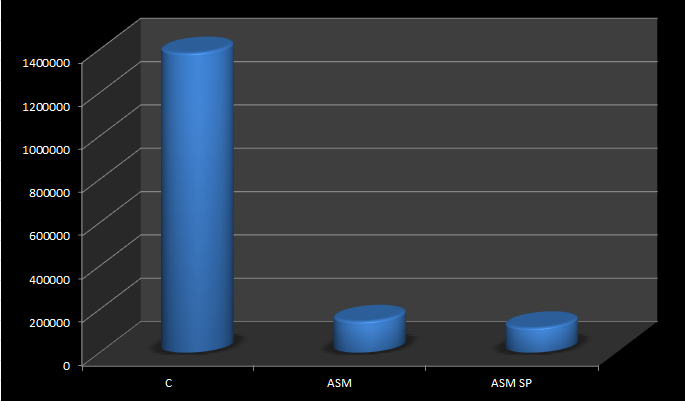
\includegraphics[scale=0.85]{imagenes/decode-resultados.png} 
\par
\bigskip
\subsubsection{Conclusiones de los resultados}
Se puede observar una mejora notable entre las versiones C y ASM, se ejecuta aproximadamente 10 veces mas rapido la version en assembler, superando las expectativas de mejora de 4 veces estimadas al comienzo de la implementacion. Asi mismo se obtuvo una mejora aproximada del $27\%$ contra el assembler original aplicando software pipelining. Lo que nos da una mejora total aproximada entre C y ASM con SP de $1200\%$






%Guardo esta cosa turbia para hacer graficos por si acaso

%\begin{figure}[H]
%    \centering
%    \begin{tikzpicture}[>=stealth]
%        % Porcentajes
%        \def\recortar  {6.43}
%        \def\halftone  {6.64}
%        \def\umbralizar{8.92}
%        \def\colorizar {2.28}
%        \def\plasma    {2.35}
%        \def\rotar     {41.17}
%
%        \def\escala    {0.2}
%
%        % Recortar
%        \filldraw[fill=gray] (1,    0) rectangle ++(1, {\recortar * \escala});
%        \draw                (1.5,  0) node[anchor=north]{Recortar};
%        \draw                (1.5, {\recortar * \escala}) node[anchor=south]{\recortar\%};

%        % Halftone
%        \filldraw[fill=gray] (3,    0) rectangle +(1, {\halftone * \escala});
%        \draw                (3.5,  0) node[anchor=north]{Halftone};
%        \draw                (3.5, {\halftone * \escala}) node[anchor=south]{\halftone\%};
%
%        % Umbralizar
%        \filldraw[fill=gray] (5,    0) rectangle +(1, {\umbralizar * \escala});
%        \draw                (5.5,  0) node[anchor=north]{Umbralizar};
%        \draw                (5.5, {\umbralizar * \escala}) node[anchor=south]{\umbralizar\%};
%
%        % Colorizar
%        \filldraw[fill=gray] (7,    0) rectangle +(1, {\colorizar * \escala});
%        \draw                (7.5,  0) node[anchor=north]{Colorizar};
%        \draw                (7.5, {\colorizar * \escala}) node[anchor=south]{\colorizar\%};

%        % Plasma
%        \filldraw[fill=gray] (9,    0) rectangle +(1, {\plasma * \escala});
 %       \draw                (9.5,  0) node[anchor=north]{Plasma};
  %      \draw                (9.5, {\plasma * \escala}) node[anchor=south]{\plasma\%};
%
 %       % Rotar
  %      \filldraw[fill=gray] (11,   0) rectangle +(1, {\rotar * \escala});
   %     \draw                (11.5, 0) node[anchor=north]{Rotar};
    %    \draw                (11.5, {\rotar * \escala}) node[anchor=south]{\rotar\%};   
%
 %       % Ejes
  %      \draw [->] (0, 0) -- +(0,  10);
   %     \draw      (0, 0) -- +(13, 0);
    %\end{tikzpicture}
    %\caption{Tiempo de ejecución de las implementaciones assembler respecto a C.}
%\end{figure}


%%%%%%%%%%%%%%%%%%%%%%%%%%%%%%%%%%%%%%%%%%%%%%%%%%%%%%%%%%%%%%%%%%%%%%%%%%%%%%%
%% Conclusión                                                                %%
%%%%%%%%%%%%%%%%%%%%%%%%%%%%%%%%%%%%%%%%%%%%%%%%%%%%%%%%%%%%%%%%%%%%%%%%%%%%%%%


\section{Conclusión}
Durante todo este trabajo, pudimos comprobar de forma empirica las ventajas que brindan las instrucciones del set SIMD provisto por Intel. A pesar de las optimizaciones brindadas por el compilador $GCC$ que mejoran de forma dramatica los resultados entre las implementaciones en C que no estan optimizadas y las versiones que si lo son, la paralelizacion de lectura y calculos para la aplicacion de los filtros, que en definitiva son procesamientos aritmeticos sobre matrices de numeros, redujeron la cantidad de ciclos requeridos para obtener un algoritmo que realice de forma correcta la transformacion impuesta por los diferentes filtros.\\
Mas alla de estos resultados favorables obtenidos, algunas de las implementaciones de los filtros en assembler con instrucciones SIMD tuvieron que ser planteadas desde otro punto de vista para un mejor aprovechamiento del set de instrucciones a nuestro alcance, lo cual nos ocasiono varias trabas a lo largo del trabajo. Luego de obtener las primeras mediciones, se realizaron sucesivas optimizaciones sobre las implementaciones de los filtros, tanto en C como en Assembler, con el objetivo de ir disminuyendo la cantidad de ciclos consumidos por estos viendose esto reflejado en los analisis publicados en este informe.

\end{document}